\documentclass[12pt]{article}
\documentclass[12pt]{article}
\usepackage[spanish]{babel}
\usepackage[square,numbers]{natbib}
\usepackage{url}
\usepackage[utf8x]{inputenc}
\usepackage{amsmath}
\usepackage{amsfonts}
\usepackage{amssymb}
\usepackage{array}
\usepackage{dsfont}
\usepackage{amsthm}
\usepackage{enumitem}
\usepackage[T1]{fontenc}
\usepackage{booktabs}
\usepackage{siunitx}
\usepackage{geometry}
\usepackage{graphicx}
\usepackage{circuitikz}
\usepackage{wrapfig}
\newcommand{\degree}{\ensuremath{^\circ}}
\usepackage{multicol}
\usepackage{fancyhdr}
\usepackage{vmargin}
\usepackage[ddmmyy]{datetime}
\usepackage{anyfontsize}
\usepackage{tikz}
\usepackage{xcolor}
\usepackage{comment}
\usepackage{setspace}
\usepackage{ulem}
\usepackage{cancel}
\usepackage{ragged2e}
\usepackage{float}
\usepackage{siunitx}
\usepackage{xfrac}
\usepackage{nicefrac}
\usepackage[autostyle]{csquotes}
\usepackage{caption}
\usepackage{listings}
\usepackage{imakeidx}
\usepackage{multirow}
\usepackage[hidelinks]{hyperref}
\usepackage{colortbl}
\usepackage{subcaption}
\usepackage{wrapfig}

\makeatletter
\renewcommand\paragraph{\@startsection{paragraph}{4}{\z@}%
  {2ex plus .2ex}%  Espacio antes
  {0.5em}%             Espacio después
  {\normalfont\normalsize\bfseries}% Estilo
}
\makeatother


% Configuración del encabezado para la carátula y el índice

\newcommand{\quotes}[1]{``#1''}

\sisetup{
  per-mode=fraction,
}

\renewcommand\indexname{Índice}

\setmarginsrb{3 cm}{2.5 cm}{3 cm}{2.5 cm}{1 cm}{1.5 cm}{1 cm}{1.5 cm}

\captionsetup{
    width=0.6\textwidth, % Ancho del caption
    margin=20pt, % Margen del caption
}

\makeindex[columns=3, title=Alphabetical Index, intoc]

\begin{document}

%--------------------------- DATOS GENERALES -----------------------------%

\title{Trabajo Profesional de Ingeniería Electrónica}	% Titulo del trabajo.
\author{UBA - Facultad de Ingeniería}	% Nombre y apellido
\newcommand{\tpnumber}{I}       % Número de trabajo práctico
\date{\today}					% Fecha (automática, no tocar)

\makeatletter
\let\thetitle\@title
\let\theauthor\@author
\let\thedate\@date
\makeatother

\pagestyle{fancy}

\fancyhead[R]{Grupo 2}
\fancyhead[L]{TP1}
\rhead{\theauthor}
\lhead{\thetitle}
\cfoot{\thepage}

%-------------------------------------------------------------------------%
%-------------------------------------------------------------------------%
%------------------------------- CARÁTULA --------------------------------%
%-------------------------------------------------------------------------%
%-------------------------------------------------------------------------%

\begin{titlepage}
\fancyhf{} % limpia encabezado y pie

% --- Configuración del pie de página ---
\fancyfoot[L]{\small Trabajo Profesional de Ingeniería Electrónica}
\fancyfoot[R]{\small Año 2026}

% --- Quita la línea del encabezado y activa la del pie ---
\renewcommand{\headrulewidth}{0pt}
\renewcommand{\footrulewidth}{0.4pt}
\thispagestyle{fancy}

\vfill 

\begin{center}
    
\includegraphics[scale=0.6]{FIUBA.png}\\[1cm]
    
    {\huge \textbf{Diseño de una plataforma experimental de ecualización activa de celdas de litio}}\\[1cm]

    {\large\textbf{Integrantes}}\\[0.2cm]
    {\Large Sebastián Ezequiel García}\\
    Padrón: 103780\\
    \textit{sebgarcia@fi.uba.ar}\\[0.3cm]
    
    {\Large Denise Oriana Viltes}\\
    Padrón: 106943\\
    \textit{dviltes@fi.uba.ar}\\[1cm]

    {\large\textbf{Tutora}}\\[0.2cm]
    {\Large Dra. Cecilia G. Galarza}\\
    \textit{cgalar@fi.uba.ar}\\[0.3cm]
    {\large\textbf{Cotutor}}\\[0.2cm]
   {\Large Ing. Juan Zuloaga}\\
    \textit{jzuloaga@fi.uba.ar}\\[1cm]
\end{center}
\vfill 
\end{titlepage}

\newpage
\tableofcontents
\clearpage


\onehalfspacing
\justifying

%-------------------------------------------------------------------------%

\section{Marco teórico}
\begin{comment}
    

-->Ver propuesta, baterias, ecualizacion pasiva y activa

1) QUE ES UNA BATERIA
2) QUE ES UN BMS -> FUNCIONES DEL BMS
3) ECUALIZACION-> PASIVA VS ACTIVA
4) SOLUCION PROPUESTA (breve porque se desarrolla bien en diseño del circuito)
\end{comment}
En la actualidad, con la creciente demanda energética, sumado a la reducción progresiva de la generación de electricidad mediante combustibles fósiles, son necesarias más y mejores forma de almacenar energía eléctrica. Las baterías de litio recargables como  Li-Ion, Li-Po, LiFePO4, etc,  demostraron ser una forma eficiente de almacenamiento.

Generalmente en la mayoría de aplicaciones en las que se requiere una bateriía, se necesita más de lo que puede suministrar una única celda. Por lo tanto, una batería es formada por un grupo de celdas, las cuales se conectan conformando una matriz que cumple con los requerimientos necesarios para el dispositivo en cuestión. Debido a variaciones en las condiciones de fabricación de cada celda, una única batería puede contener celdas con diferentes capacidades \cite{chen2015system}, distintos coeficientes térmicos o, incluso distinto envejecimiento . En cada carga y descarga, estas diferencias provocan desbalances en las carga almacenada en cada celda, parámetro conocido como SoC (\textit{State of Charge}) provocando \cite{rumpf2018influence}:

\begin{itemize}
    \item Disminución de la eficiencia,
    \item Reducción en la vida útil,
    \item Sobrecalentamiento,
    \item Riesgo de cortocircuitos por formación de filamentos de litio metálico.
\end{itemize}



Para mitigar estas complicaciones, el BMS, \textit{Battery Management System}\cite{quinones2019estudio}, debe cumplir el rol de garantizar un funcionamiento seguro de la batería protegiendo las celdas de sobrecarga, sobredescarga y sobrecorriente, asimismo mantener las condiciones seguras de operación dentro de los rangos adecuados de tensión y  temperatura y asi  prolongar la vida útil de las baterías todo lo posible,  En este contexto surge la necesidad de distribuir la energía de forma equitativa en toda la batería y así aprovechar la capacidad total de la misma \cite{lu2013review}. Para ello, la técnica de ecualización resulta una herramienta necesaria, y se puede clasificar en dos tipos de métodos, pasivos o activos, basándose en la topología del sistema. Se ecualiza a partir de una de las características de la batería como, el Soc, la tensión o la capacidad \cite{hua2020comprehensive}.

\begin{comment}
    cuadrito de metodos de ecualización?
\end{comment}

Los métodos pasivos son los más ampliamente difundidos por su simplicidad, fiabilidad y bajo costo. Suele tratarse de un \textit{shunt} resistivo conectado en paralelo a la batería para disipar el exceso de energía de las celdas. Este método aunque es simple y de baja complejidad, trae como desventaja una gran duración de ecualización debido a la baja energía de ecualización y también una corriente de balanceo restringida a los limites de disipación de calor del propio hardware , limitando el uso de este tipo de ecualización, principalmente en baterías de gran capacidad\cite{hua2020comprehensive}.Muchos de estos inconvenientes son posibles solucionar mediante ecualización activo pero aumentando la complejidad de y costo del circuito \cite{pericsoarua2018passive}.

\begin{comment}
    agregar imagen como ejemplo de la conexión del shunt
\end{comment}

Los circuitos de ecualización activa tienen una topología que no utiliza la disipación de la energía sobrante de una celda en su lugar, se transfiere la energía sobrante de una celda a otra celda del circuito o módulos utilizando componentes capaces de almacenar energía como, capacitores, inductores, transformadores, y convertidores,



%se requiere contar con un sistema de control que se encargue de medir el estado de cada celda y del balance de cargas para optimizar el desempeño general del sistema. A este controlador se lo denomina BMS, \textit{Battery Management System}, cuya tarea principal es la ecualización de las cargas . De esta forma se logran diversas estrategias como un \textit{shunt} resitivo para disipar la energía sobrante (balanceo pasivo \cite{li2023active}), convertidores DC-DC, capacitores conmutativos (balanceo activo \cite{li2023active}), entre otras tecnologías \cite{chen2015system}.







\input{Capitulos/Diseño del circuito}
\section{Prototipo}

[Matriz $3\times2$, uso de celdas 18650 de \SI{3.2}{\volt}]

[PONER LAS MEDICIONES Y EL TESTEO COMO OTRA SECCION]

[AGREGAR UN APENDICE CON UN PEQUEÑO MANUAL DE USO DEL CIRCUITO]

\subsection{Diseño del prototipo}

[Uso de una fuente externa para los LEDs e inversores]
[ejamos el capatitor en una bornera en la salida para  ver cual sirve en la realidad]

\subsubsection{Diseño del esquemático}

[LEDs, portapilas, fusibles, \textit{test points}, \textit{jumpers}]

[POR QUÉ DISEÑAMOS ASÍ LA PLACA, ESPACIO, DISPOSICIÓN, ETCÉTERA]

\subsubsection{Diseño del PCB}

[Placa de $\SI{20}{\centi\meter}\times\SI{20}{\centi\meter}$ bifásica]





////////////


\subsection{Controlador para el prototipo}

[Selección de microcontrolador]



\subsubsection{Diseño del controlador para el prototipo}

[Primero se apaga lo que se deba apagar y después se enciende lo que se deba encender]
 
Para programar el controlador se utiliza la aplicación \textbf{\textit{STM32CubeIDE}}, este entorno permite desarrollar, compilar y depurar el código del microcontrolado, en este caso, \textbf{STM32 NUCLEO-F103RB}. Para la configuración inicial de la placa se utiliza la aplicación \textbf{\textit{STM32CubeMX}}, con la cual se crea el archivo \textit{.ioc}, almacenando toda la información de la configuración de los pines, y todos los archivos necesarios para el funcionamiento de la placa. En la STM32CubeMX
se configura la función de los pines, se habilitan los pines necesarios y se configura de ser necesario el clock, DMA, interrupciones, etc. Uno de los archivos que se generan, es el \textit{main.c}, donde se inicializan todos los periféricos, también proporciona el bucle principal \textit{while(1)}, en donde se pueden agregar las tareas principales.

 En el prototipo, el enfoque principal es diseñar el control manual para probar cada configuración de la matriz. Se utiliza el control manual para poder acceder y probar cada celda, este modo sirve para imitar las simulaciones en \textit{LTSpice} y evaluar el comportamiento del prototipo. 
 En una primera instancia se simplifica el diseño del controlador a determinar el estado de cada celda mediante linea de comandos (CLI), y a partir del estado de todas las celdas del banco, el controlador actualiza el estado del switch del banco según corresponda.
 
 Para este diseño cada switch es un pin distinto del microcontrolador, esto significa que se deben reservar 1 pin para switch del banco y 1 pin para el switch de la celda, resultando en 9 pines \textit{gpio} en modo salida para el prototipo. Cada pin se enciende o se apaga determinando su estado a través del HAL.
 

Otro requerimiento es la posibilidad de probar el \textit{modo de switching}, en este estado se espera poder encender y apagar los apagar los pines de forma alternada, permitiendo evaluar la conmutación entre celdas y entre bancos. No se espera que el sistema conmute a altas frecuencias en condiciones normales, pero si es necesario verificar como responde el sistema ante este caso. Por lo tanto, el programa del controlador debe tener la posibilidad de asignar el estado \textbf{\textit{switching}} a una celda, siempre actualizando de forma acorde el switch del banco. Se proponen dos opciones, switching sincronizado y complementario, para lograr esto se asignan flags a cada celda seleccionada y se actualiza de forma simultanea todos los pines. Al mismo tiempo, desde el CLI, se le asigna un grupo a cada celda, cada grupo responde a la frecuencia elegida. De esta forma se permite testear conmutación entre celdas, entre bancos, el sistema a distintas frecuencias, y grupos de celdas a distintas frecuencias, así como encontrar los limites en frecuencia del sistema.

Cabe destacar que para obtener una representación fiel de la frecuencia pedida, es necesario actualizar el estado según una base temporal constante. Para ese se puede utilizar el \textit{\textbf{SysTick}}, un temporizador integrado, el cual genera interrupciones periódicas cada \SI{1}{\milli \second}. Para utilizar esta base, se coloca la función correspondiente a la actualización de los pines dentro de la rutina de interrupciones, \textbf{$SysTick_Handler()$} así actualizando el estado de la matriz de forma regular. En caso de utilizar el bucle principal en \textit{main.c}, no se obtendría una base temporal constante, ya que la duración de una iteración depende de la duración del resto de las tareas.


[AGREGAR FOTITO DEL PUTTY]




\subsection{Implementación}

[DECIR QUE ESTABA \enquote*{MAL} LA HUELLA DEL PMOS]

\section{Mediciones sobre el prototipo}

[VER SI ESTÁ BIEN SEPARAR EN IMPLEMENTACIÓN Y MEDICIONES O HACERLO TODA UNA MISMA SECCIÓN]

Como se mencionó previamente, el objetivo del prototipo era verificar el correcto funcionamiento del circuito real. Para eso la etapa de medición es crucial, dado que se puede utilizar para buscar posibles errores y mejoras a implementar en el dispositivo final. Sin embargo, como medida cortafuegos, se decidió soldar el prototipo y medir de forma progresiva: primero una celda, luego un banco, y finalmente todo el circuito. De este modo, en caso de haber alguna falla crítica, se puede detectar de forma temprana antes de ya haber dedicado más trabajo y usado todos los componentes a disposición.

\subsection{Primera medición fallida en una celda del banco 1}

Lo primero que se soldó fue el circuito de una de las celda junto con la etapa de control del banco $1$. Aunque a simple vista parecía que todo estaba en orden, rápidamente se reveló que no era el caso.

[INSERTAR IMAGEN DEL KICAD Y FOTO DE ESTA CELDA]

En primer lugar se buscó verificar el funcionamiento en estado estacionario de la celda, por lo que se conectó a la entrada una fuente de tensión continua de \SI{5}{\volt} (con una corriente de hasta \SI{20}{\milli\ampere}). Esto debería ser suficiente para obtener como tensión de salida a la de la celda pero no fue el caso: la salida era nula con pequeñas variaciones ocasionales en torno a las decenas de milivolts.

Ante la temprana falla se midieron las caídas de tensión de todos los componentes en las mallas de control. Cuando se estaba midiendo la caída sobre el resistor $R_3$, el TBJ PNP $Qij_2$ comenzó a soltar humo. De este punto en adelante se desataron una serie de eventos desafortunados que concluyeron en el reemplazo de varios componentes más.

En el intento de desoldar el transistor para reemplazarlo, el diodo \textit{zener} también empezó a soltar humo. Fue tanta la temperatura que desprendió que el estaño que lo sujetaba se fundió. Cabe destacar que la fuente de continua no estaba conectada pero sí estaba colocada la celda. Aunque debido a la baja potencia que emite, ésta no debería haber sido la causa de la destrucción del diodo.

Luego, más humo se desprendió de lo que parecería ser el fusible de la celda. Éste fue rápidamente extraído, aunque luego de unas pruebas con multímetro se descubrió que ambos fusibles estaban perfectamente bien y que ninguno se había quemado.

Dado este nuevo suceso, se decidió que lo más probable que se haya quemado era el transitor N-MOSFET de la tierra, por lo que se lo desoldó. Debido a la proximidad con otros componentes, el calor del soldador fue tal que el plástico del portafusible de la celda se derritió. No hubo otra opción que también descartarlo, siendo el cuarto componente en seguidilla en ser eliminado y sin tener una clara idea de cuál fue el problema.

\subsection{Segundo intento de medición y primero exitoso}

Luego de los problemas del intento anterior, se priorizó restaurar los componentes en la placa, asegurándose en cada paso el correcto funcionamiento de los mismos. Comenzando por la etapa de control, se soldaron nuevos TBJ NPN y diodo \textit{zener}. Ingresando una tensión de control equivalente a un $1$ lógico (\SI{5}{\volt}) se corroboró la correcta apertura del transistor.

Luego, debido a la proximidad de los componentes y el gran tamaño relativo de los portafusibles, se decidió extraerlos. En su lugar se colocaron alambres para cerrar las mallas en las que estaban colocados.

Con lo soldado hasta ahora el sistema debería prender y apagar correctamente la celda. Lo único faltante es el N-MOSFET de la tierra. Cuando se lo desoldó, la pista quedó dañada y se soltó el \textit{pad}, por lo que colocarlo nuevamente resultaría dificultoso. Más adelante es algo que debe hacerse (y se hizo) pero por el momento se podría medir sin el transistor y cortocircuitar la tierra con el nodo correspondiente de forma manual con cables cuando sea necesario.

Con el circuito de la celda devuelto a casi su estado original se conectó todo para volver a medir. Cabe destacar que en lugar de la celda de litio se colocó una tensión a través de una fuente de continua. La razón detrás de esta decisión fue colocar una corriente máxima de \SI{100}{\milli\ampere} para, en caso de que algo falle, minimizar la probabilidad de quemar más componentes.

Con todo esto en mente, se encendieron las fuentes que emiten la tensión de la celda y la entrada de control y se obtuvo a la salida la tensión de la celda. Aunque un progreso respecto del último intento de medición, rápidamente se hizo notorio otro problema: la fuente de la celda estaba emitiendo corriente. Normalmente eso es lo que se esperaría ver salvo cuando la salida está abierta (como era el caso en cuestión) donde no debería haber corriente circulando. Estos valores rondaban los \SI{80}{\milli\ampere} o \SI{90}{\milli\ampere}, valores para nada despreciables. 

Midiendo la caída de tensión en cada componente se encontró la ubicación del problema: había caída de tensión en los resistores $R_7$ y $R_8$ correspondientes a la etapa de control del \textit{switch} del banco. En ellos caían [PONER VALOR TENSIONES].

[AGREGAR IMAGEN CON EL REDONDEL ROJO DE LOS RESISTORES EN CUESTIÓN]

Ese bloque estaba apagado por lo que no debería haber corriente circulando por sus componentes. Testeando continuidad en el nodo de [LA FIGURA QUE FALTA ARRIBA] hay un cortocircuito con tierra. Se desoldó el TBJ, el cual se partió a la mitad. Probablemente haya estado quemado, lo cual explicaría el humo visto previamente en el primer intento de medición que se había creído erróneamente que provenía de alguno de los fusibles. El cortocircuito seguía estando por lo que también se extrajo el JFET, momento en el cual se solucionó el problema.

Nuevamente se incorporan las fuente de tensión y esta vez sí se obtiene el resultado esperado: \SI{33.}{\volt} a la salida con corriente nula. Incorporando cargas de prueba se aprecia que la corriente de salida varía. El MOSFET de la tierra flotante sigue ausente pero se pudo corroborar el correcto funcionamiento del encendido y apagado de una celda.

\subsection{Problemas de diseño del prototipo}

Entre mediciones fallidas y valores no esperados, se pudieron identificar algunos errores de diseño. Por un lado por huellas mal elegidas, y por otro, por errores en el esquemático. Antes de detallarlos es importante destacar que ninguno de estos problemas son críticos ni inhibieron el circuito. Aunque simples de corregir para la versión final, requirieron de trabajo y tiempo al momento de identificarlos.

En primer lugar se tienen los problemas en las huellas, comenzando por la de los JFET. Debido a una confusión con los TBJ, los cuales usan el mismo encapsulado pero diferente configuración de los pines, la huella en \textit{KiCad} no coincidió con la dada en la \textit{datasheet}, como se muestra en la figura \ref{fig:JFET_pinout}.

\begin{figure}[H]
    \centering
    \begin{subfigure}{0.3\textwidth}
        \centering
        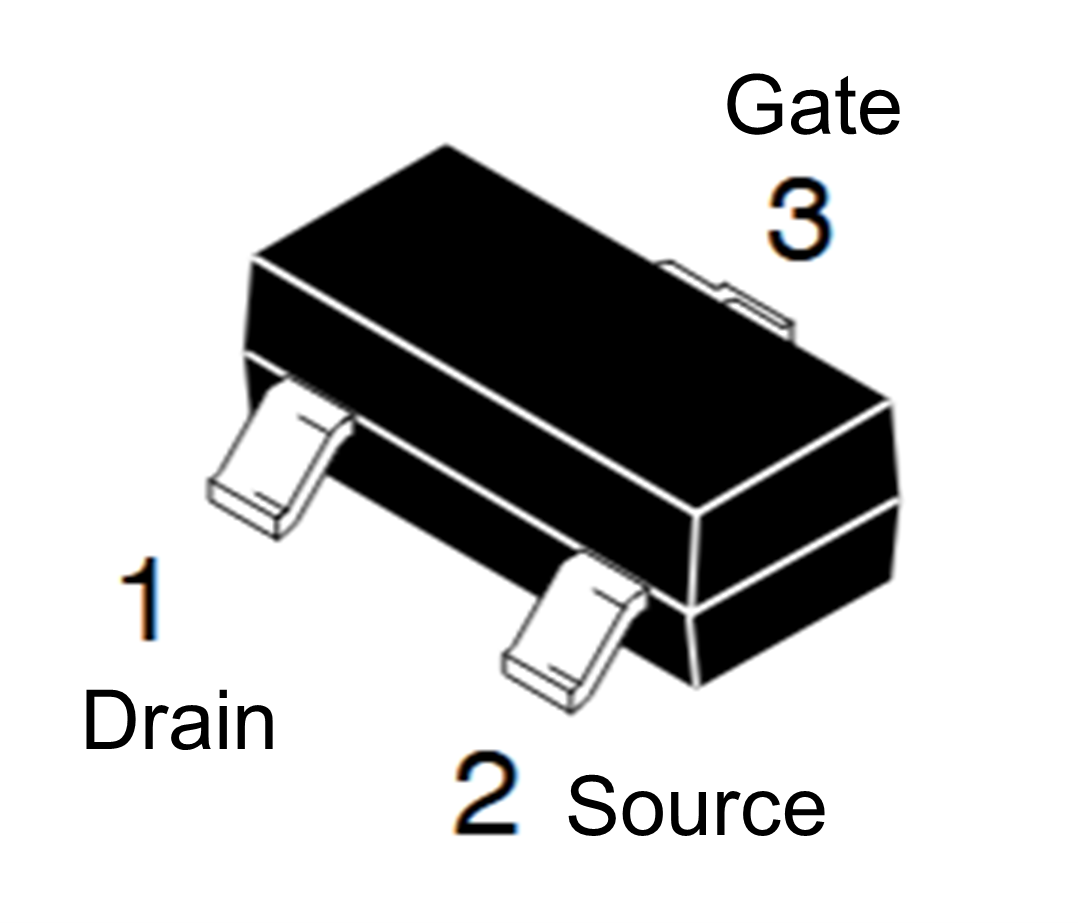
\includegraphics[width=\linewidth]{Imágenes/Prototipo/JFET pines con nombre.png}
        \caption{}
        \label{fig:JFET_pinout_datasheet}
    \end{subfigure}
    \hfill
    \begin{subfigure}{0.4\textwidth}
        \centering
        
\includegraphics[width=\linewidth]{Imágenes/Prototipo/JFET pines con nombre KiCad.png}
        \caption{}
        \label{fig:JFET_pinout_kicad}
    \end{subfigure}
    \caption{\textit{Pinout} del JFET MMBFJ201 según la hoja de datos (a) y como fue configurado en la huella de \textit{KiCad} (b).}
    \label{fig:JFET_pinout}
\end{figure}

De forma similar, la huella de los diodos \textit{zener} estaba invertida. Esto significó una inversión del ánodo y el cátodo como se aprecia en la figura \ref{fig:zener_kicad}.

\begin{figure}[H]
    \centering
    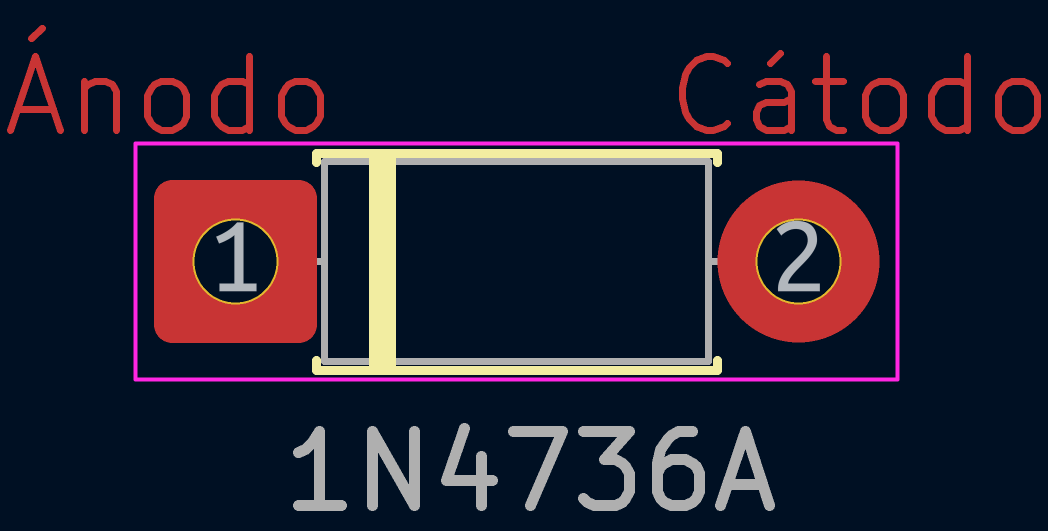
\includegraphics[width=0.4\linewidth]{Imágenes/Prototipo/Diodo KiCad.png}
    \caption{Huella del diodo \textit{zener} utilizada en \textit{KiCad}.}
    \label{fig:zener_kicad}
\end{figure}

Siendo un elemento de protección, no tiene un rol activo en el funcionamiento del circuito, es más, si todo se desarrolla correctamente nunca debería actuar. Pero el hecho que se encuentre en directa conduciendo cuando no debería provocó valores altos de tensión en el nodo del \textit{gate} de los N-MOSFET cuando el sistema está apagado.

[PONER DIAGRAMA DE LA MALLA DEL CIRCUITO Y COMPLETAR]
[ESTA BIEN DECIR QUE LA TENSION ERA DE 3.3-0.7 EN EL GATE CUANDO ESTABA APAGADO?]

Por otro lado, se tiene la huella de los P-MOSFET. Aunque técnicamente era la huella correcta, la hoja de datos da un comentario que no se tuvo en cuenta. En la figura \ref{fig:pmos_config_datasheet} se ve que hay una región que debería estar libre de cobre en la placa, indicada como "KEEP OUT AREA".

\begin{figure}[H]
    \centering
    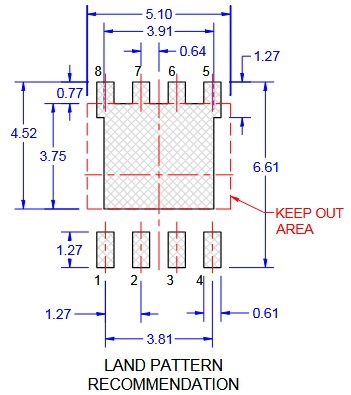
\includegraphics[width=0.5\linewidth]{Imágenes/Prototipo/PMOSFET huella datasheet.jpg}
    \caption{Vista inferior del transistor P-MOSFET FDMS6681Z mostrada en su \textit{datasheet}.}
    \label{fig:pmos_config_datasheet}
\end{figure}

Al no incorporar esa zona, hubieron complicaciones al momento de soldarlo: hicieron falta varios intentos de soldar y desoldar el transistor para evitar que el \textit{drain} entre en cortocircuito con el plano de tierra. Finalmente, lo que se decidió hacer es con un destornillador raspar parte del cobre y así evitar que entre en contacto con el MOSFET, como se muestra en la figura \ref{fig:pmos_arreglado}.

\begin{figure}[H]
    \centering
    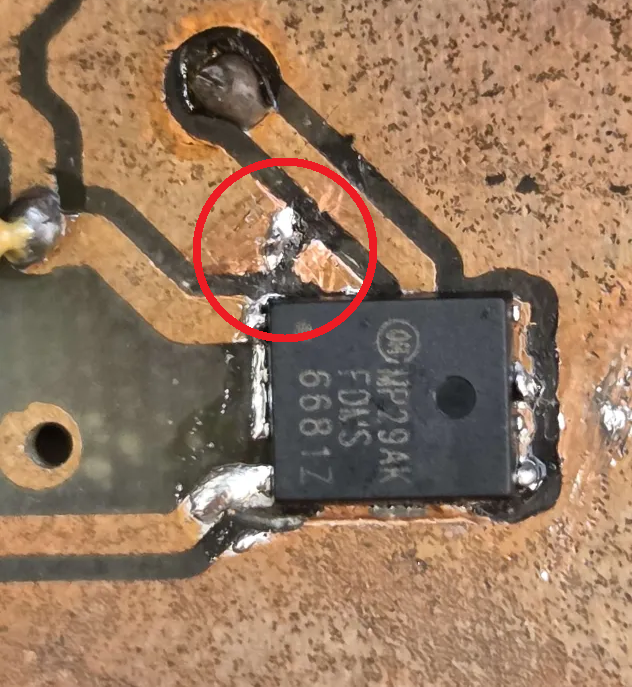
\includegraphics[width=0.4\linewidth]{Imágenes/Prototipo/PMOS arreglado.png}
    \caption{Foto del transistor P-MOSFET FDMS6681Z soldado indicando la corrección que se hizo para que no haya cortocircuito entre el \textit{drain} y el plano de tierra.}
    \label{fig:pmos_arreglado}
\end{figure}

Al margen de los errores de huellas, hubo otro error menor de diseño con el \textit{jumper} del primer banco. Recordemos que se incorporaron \textit{jumpers} para cada banco, de forma que se pueda medir por separado cada uno usando siempre la misma bornera como salida para colocar carga. Sin embargo, para el primer banco, fue mal diseñado como se aprecia en la figura \ref{fig:jumper_mal}.

\begin{figure}[H]
    \centering
    \begin{subfigure}{0.45\textwidth}
        \centering
        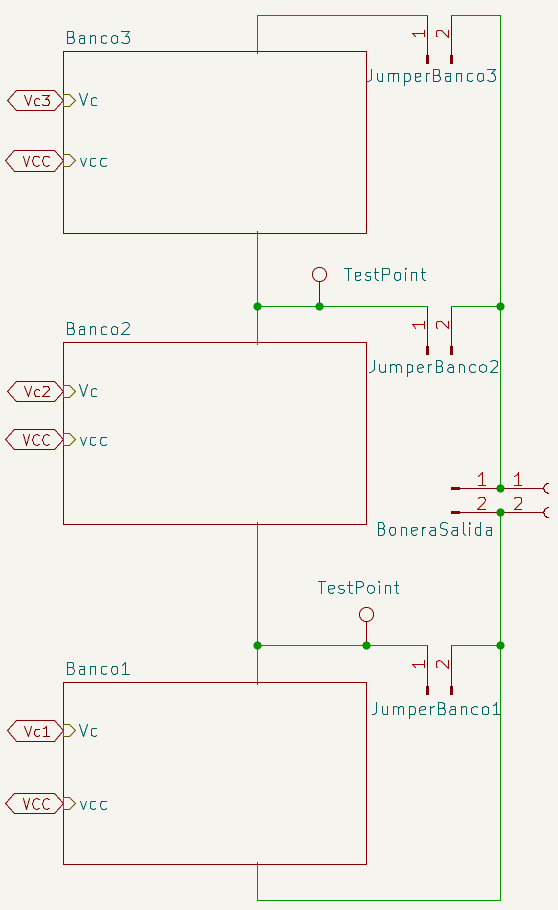
\includegraphics[width=\linewidth]{Imágenes/Prototipo/Jumper Mal.png}
        \caption{}
        \label{fig:jumper_mal}
    \end{subfigure}
    \hfill
    \begin{subfigure}{0.45\textwidth}
        \centering
        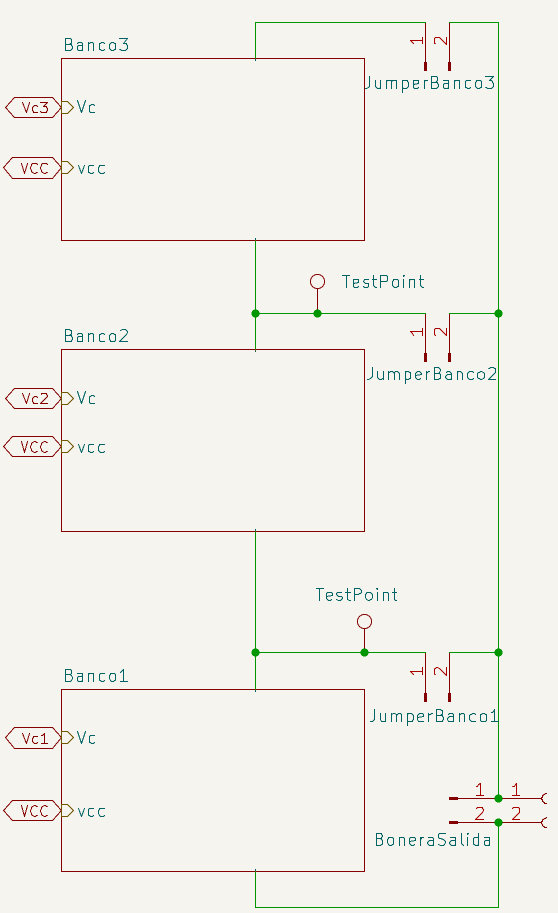
\includegraphics[width=\linewidth]{Imágenes/Prototipo/Jumper Corregido.png}
        \caption{}
        \label{fig:jumper_bien}
    \end{subfigure}
    \caption{Esquema de cómo fue diseñado el circuito prototipo erróneamente en \textit{KiCad} (a) y cómo debería haber sido (b).}
    \label{fig:jumpers}
\end{figure}

El objetivo de los \textit{jumpers} era poder seleccionar si la tensión de la bornera de salida correspondía a una de tres opciones: solo el banco 1, los bancos 1 y 2, o los tres bancos. Sin embargo, como fue diseñado el circuito, el \textit{jumper} correspondiente al primer banco no tenía función alguna, y, en caso que se conecte, se estaría poniendo peligrosamente en cortocircuito a las celdas.

Otro inconveniente fue la forma en la que se soldaron los transistores N-MOSFET. Con el objetivo de minimizar el uso de vías, se utilizaron algunos de los componentes THT para conectar pistas entre capas opuestas. Esto fue práctico usando resistores y diodos pero no fue buena idea con los transistores. Debido a tener pines gruesos, a la forma del encapsulado y a la ubicación en la placa, soldar en la capa \textit{front} resultó incómodo. Como consecuencia de esto, las soldaduras quedaron desprolijas y se torna complicado el proceso de desoldado si fuera necesario.

Por último, el mayor problema que tuvo la placa fue una pobre elección de P-MOSFET como \textit{switch} del circuito \textit{by-pass} de banco. Cuando el transistor debía estar encendido, la tensión $V_{GS}$ era de alrededor de $\SI{1.8}{\volt}$, sin embargo, la tensión de umbral típica (extraída de su hoja de datos) es de $\SI{1.7}{\volt}$. Esto quiere decir que, aunque tecnicamente el MOSFET estaba conduciendo, lo hacía con una resistencia $R_{DS}$ alta entre \textit{drain} y \textit{source}. Es por esto que se veían valores más bajos de lo esperado en la salida: unos $\SI{400}{\milli\volt}$ caen en cada uno de estos transistores cuando están encendidos. Es por esto que se decidió cambiarlo para el circuito final.




Problemas que recordamos:
    - X Huella JFET (corto en la fuente de tensión)
    - X Huella PMOS (corto de drain con tierra)
    - X Huella del Zener (casualidad)
    - X Jumper del banco 1 esta mal puesto
    - X NMOS con soldaduras en las dos capas
    - El PMOS no era correcto
Seguir investigando:
    - Zener funciona raro (no permite que el gate llegue a 0V)
            






\section{Circuito final}

Con la confirmación de funcionamiento del prototipo, se prosiguió al diseño del sistema final. La principal premisa del trabajo es que sea modular, por lo que se optó por numerosos circuitos pequeños en lugar de uno solo grande como fue el prototipo. En un principio se pensó en mantener las celdas con los portapilas en una placa por separado del resto del circuito dado el tamaño que le agrega a cada módulo. Sin embargo, finalmente se descartó esa idea, resultando en tres circuitos diferentes:

\begin{enumerate}
    \item Circuito de celdas: cada una es un módulo que alberga el portapilas, con su \textit{switch}, LED e inversor.
    \item Circuito de bancos: con el \textit{switch by-pass} de las celdas y desde donde se envían las señales de control a todas las celdas del mismo banco.
    \item Circuito central: donde se inserta el controlador y desde donde parten las señales de control a todo el sistema, y a donde llegan las señales de censado de las celdas.
\end{enumerate}

\begin{figure}[H]
    \centering
    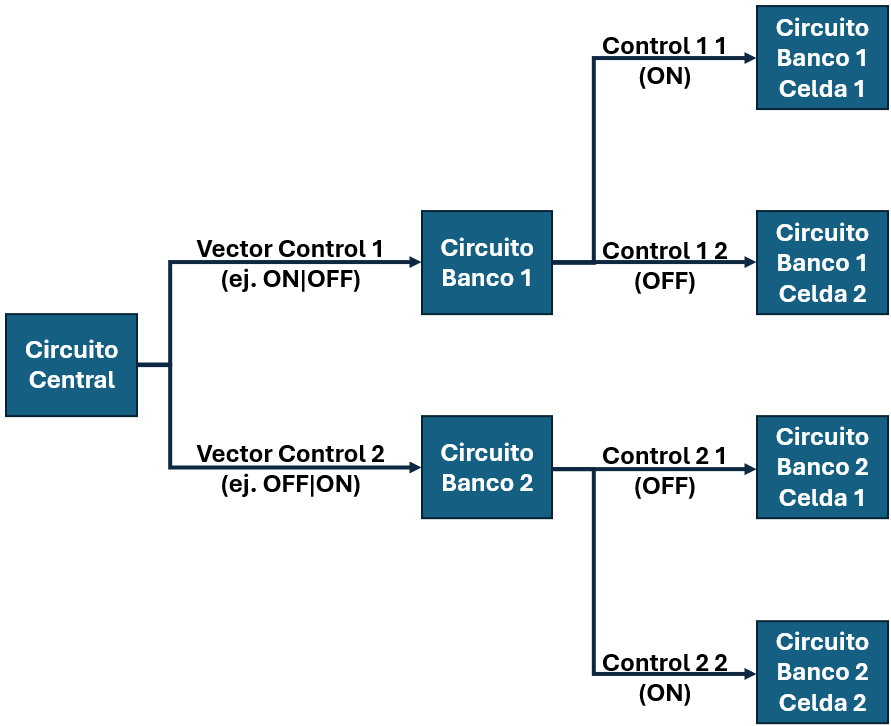
\includegraphics[width=0.7\linewidth]{Imágenes/Diseño final/Esquema de envío de señales de control.png}
    \caption{Diagrama de transporte de señales de control entre los módulos.}
    \label{fig:esquema_seniales_control}
\end{figure}

De esta forma, se armaron doce circuitos de celdas, cuatro circuitos de banco y un circuito central.

Al margen de los cambios de diseño del \textit{hardware}, también sufrió cambios el controlador. Debido a la mayor cantidad de celdas en comparación con el prototipo, son necesarios muchos más pines del controlador, más de los disponibles. Esto implica un cambio de lógica al momento de enviar las señales para maximizar el uso de cada pin de salida de la placa programable.

Al no alcanzan los pines del controlador para todas las señales que debe enviar si fuera una por cada celda, se optó por enviar la información en serie para todas las celdas de un banco. Para este rol fue que se utilizó un \textit{shift-register} con \textit{latch} (SR). Más información sobre este componente se provee en la sección del diseño de circuito de banco.

Por otro lado, otro objetivo que se planteó fue el de armar todos los circuitos, siempre que sea posible, con componentes SMD. De esta forma, buscamos:
\begin{itemize}
    \item Minimizar el área de placa de cobre usada,
    \item Facilitar el planchado y perforado de las placas,
    \item Identificar de forma clara qué corresponde a una entrada y/o salida, y qué al circuito propio de cada módulo,
    \item Aprender a soldar componentes SMD.
\end{itemize}

Otro punto a destacar fue que se decidió acerca de qué topología conformarían los módulos conectados. Ya haciendo pruebas y mediciones con el prototipo mismo, rápidamente se mostró la incomodidad al tener que usar cables \textit{dupont} para todo el conexionado. Cables demasiado largos, fácil de enredarse y que no enganchan con firmeza, complican mucho la instalación del banco de prueba. Para esto es que se decidió eliminar el uso de cables individuales y utilizar más que nada pines que encastren entre los módulo para conectarlos.

A la primera configuración planteada se la denominó "tren". Consistía en usar pines $90^\circ$ macho a un lado de la placa y hembra en el extremo opuesto. De esta forma, podrían conectarse de costado cada módulo. Sin embargo, esta configuración tenía tres grandes problemas. Por un lado, los pines hembra y macho $90^\circ$ no están a la misma altura, por lo que se tendría que soldar de forma muy cuidadosa para garantizar un encastre correcto. A su vez, el hecho que haya señales compartidas entre todas las celdas de un mismo banco implicaría que la señal entra por un costado de la placa y tendría que trasladarse a través de todo el circuito hasta la salida en el otro extremo para que el siguiente módulo reciba la señal correcta. Esto complicaría enormemente el ruteo de la placa. Por último, si se tuviera un banco con varias placas de celda, sería necesario mucho espacio en una mesa y sería complicado moverlas sin necesidad de desconectarlas. Por todo esto fue que se decidió optar por la segunda configuración.

La otra opción era la configuración "torre". Este caso era mucho más simple: los módulos de celdas se montarían uno encima de otro mediante pines y, abajo de todo como si fueran los cimientos, estaría el módulo del banco. Esto facilitaba en gran medida el ruteo (no hace falta trasladar la señal de entrada de un lado a otro de la placa), el transporte y el espacio necesario. La única condición estrictamente necesaria es que el pin macho que recibe las entradas desde el "piso de abajo" tenga un equivalente hembra apuntando hacia arriba para transmitirlas hacia el siguiente módulo. Para esto se usaron los pines hembra-macho o también llamados pines hembra largos de la figura \ref{fig:pin_hembra_largo}. Otro inconveniente menor es la poca rigidez estructural de la torre, pero se asumió que los pines tienen un agarre suficientemente fuerte como para mantener a las placas en pie. Con todos los problemas solucionados, esta configuración torre fue la elegida.

\begin{figure}[H]
    \centering
    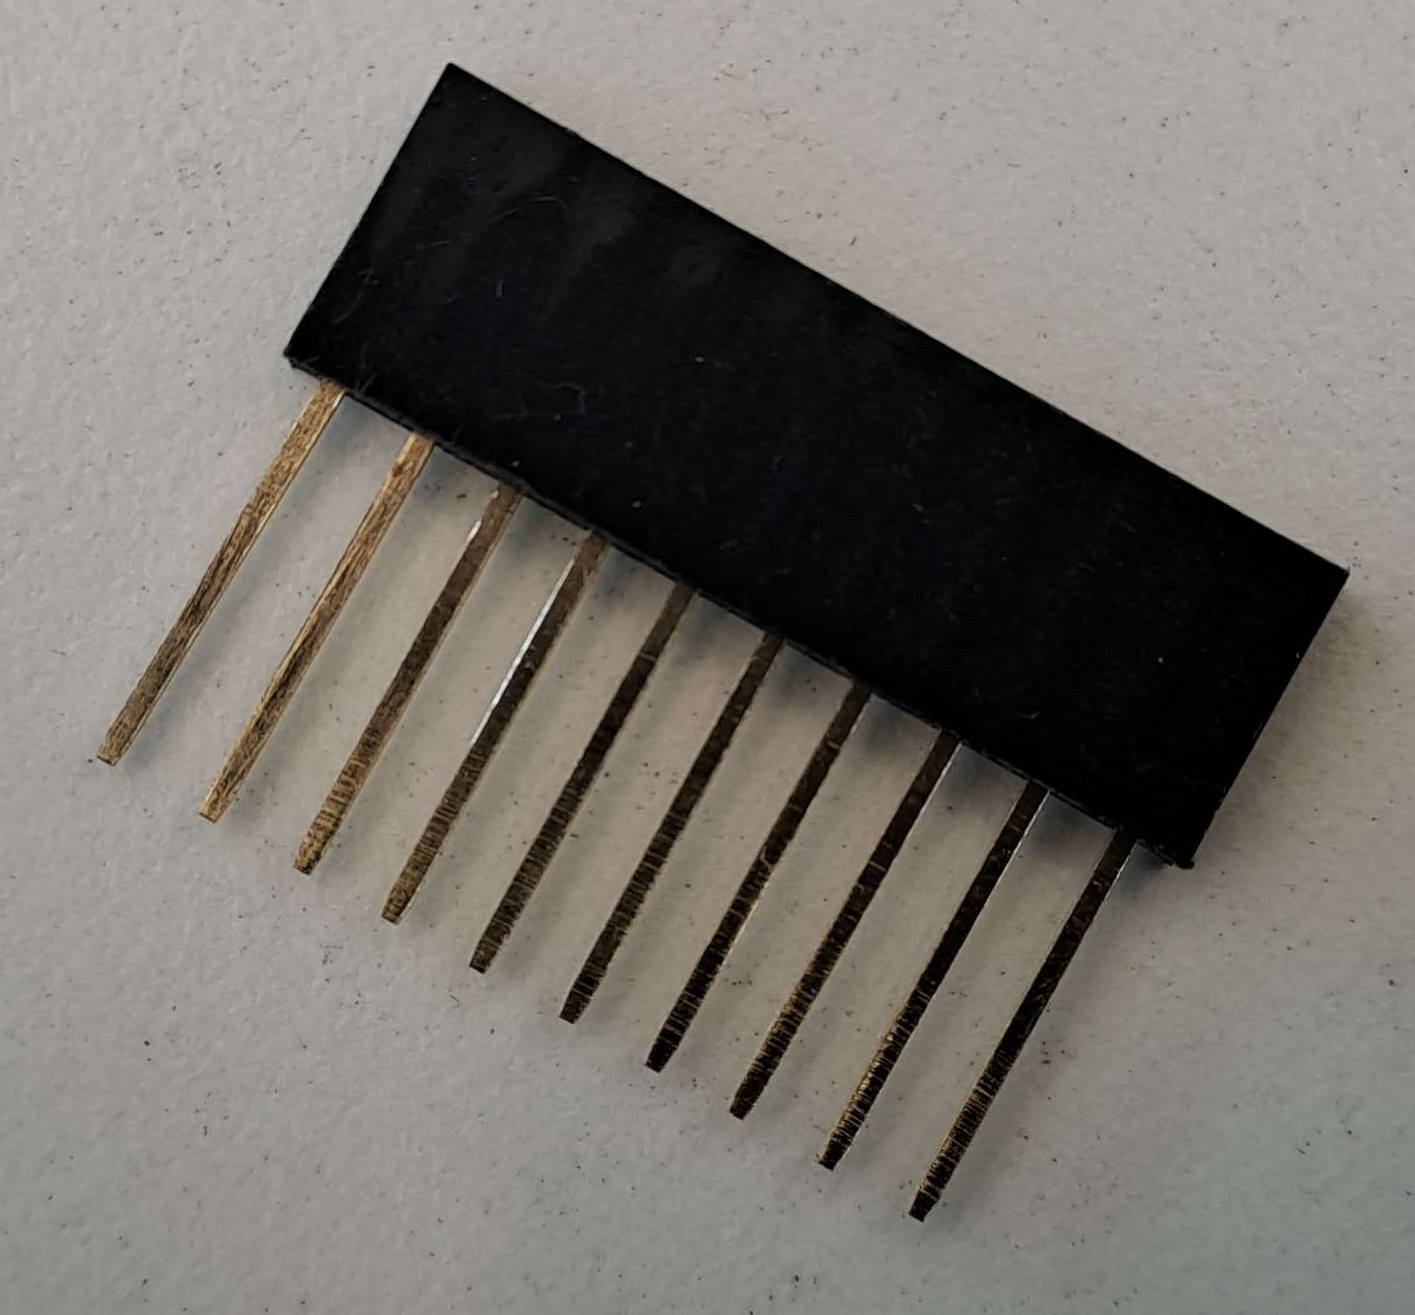
\includegraphics[width=0.4\linewidth]{Imágenes/Diseño final/Celda/Pines macho largos.jpg}
    \caption{Tira de diez pines hembra-macho utilizados.}
    \label{fig:pin_hembra_largo}
\end{figure}

\subsection{Diseño del circuito de las celdas}

%OPCIONES PARA LAS ENTRADAS A LAS CELDAS:
%- MULTIPLEXOR
%- SHIFT REGISTER CON LATCH
%- MICRO EN CADA CELDA

El principal problema a tratar fue el de los pocos pines del controlador. Antes de utilizar el \textit{shift-register}, se pensó en colocar un microcontrolador en cada módulo de celda. De esta forma, mediante comunicación I2C se podría enviar la señal de encendido o apagado a cada módulo utilizando solo dos vías. Esto permitiría conectar la cantidad de celdas que se deseen por banco. Sin embargo, se descartó esta idea debido al aumento de precio que implica y su complejidad de implementación. Finalmente se terminó optando por el envío de información en serie en una etapa anterior, y que cada módulo de celda simplemente reciba como entrada su señal de control.

\subsubsection{Versión 2.0}

El circuito, en grandes rasgos, se mantuvo como en el prototipo, al menos en cuanto a su funcionamiento. Sin embargo, sí hubieron diferencias constructivas en pos de la modularidad del sistema. El circuito propiamente dicho fue igual salvo por la incorporación de un inversor para la señal de control negada, como entrada en la base del transistor $Q_3$.

En el prototipo, para las señales negadas se utilizó el integrado \textbf{CD40106} que contenía seis inversores. En este caso, sería un desperdicio de recursos y espacio montar uno de esos por módulo, por lo que se identificaron dos opciones: tener tanto señal de control como señal negada como entradas, o incorporar un inversor más simple por módulo. Se optó por la segunda opción, y, ante la imposibilidad de conseguir inversores individuales, se implementó un inversor CMOS discreto. Para esto se utilizaron los MOSFETS \textbf{AO3400} (canal N) y \textbf{AO3401} (canal P), como se muestra en la figura \ref{fig:inversor_cmos}.

\begin{figure}[H]
    \centering
    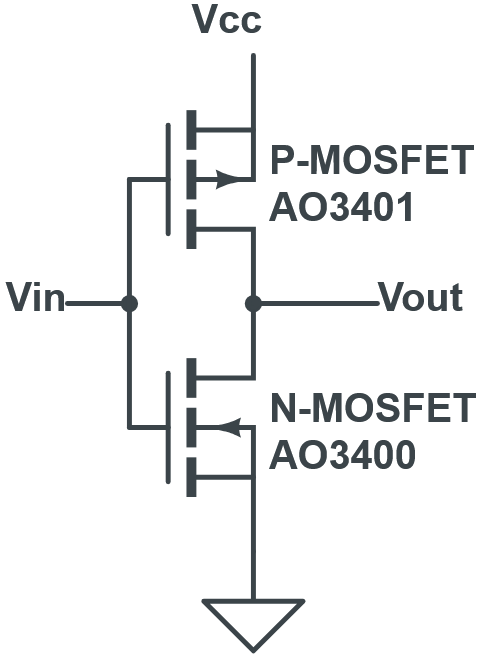
\includegraphics[width=0.3\linewidth]{Imágenes/Diseño final/Celda/Diagrama inversor CMOS.png}
    \caption{Diagrama del inversor CMOS discreto implementado.}
    \label{fig:inversor_cmos}
\end{figure}

Al igual que en el prototipo, se implementó un pequeño circuito con un LED. Mediante un TBJ NPN, se abre o cierra la malla del dispositivo según sea la señal de control del \textit{switch} de la celda. De esta forma, se puede ver claramente cuándo es que cada celda está encendida.

Cada módulo tiene una cantidad de entradas definidas para poder funcionar correctamente. En un principio están $Vcc$ y $GND$. Por un lado, necesarios para la etapa de control del módulo, la malla del LED y el inversor CMOS, y por otro para que las tierras de todos los circuitos estén acopladas. A su vez están los buses positivo y negativo de cada banco ($bus\_pos$ y $bus\_neg$). Éstos son tanto entrada como salida: si la celda está prendida, ésta impone su diferencia de tensión entre estos buses, pero a la vez, también deben coincidir con los buses de todas las celdas del banco dado que están en paralelo. Finalmente se tiene el control global. Éste es una señal de control separada de las individuales para cada celda. Con el objetivo de simplificar la comunicación, se decidió enviar, además de las señales de control individuales para cada módulo, una señal compartida para todas ellas. Dado que el control se hace por banco y no por celda, éste sería el control utilizado en el funcionamiento normal del sistema. Para poder seleccionar entre esta señal global y la individual, se usa un \textit{jumper}.

Con respecto a la entrada de control individual, se hicieron varias consideraciones. En un principio, como cada módulo envía al siguiente exactamente la misma información que recibe, cada módulo necesariamente tiene que recibir las señales de control de todas las celdas individuales del banco. Para esto se utilizó una tira de siete pines hembra-macho, uno por módulo de celda en el banco. La tarea de asignar qué señal se corresponde a qué módulo se dejó para hacerse a mano. Esto se hizo mediante una tira de pines macho dobles y un \textit{jumper}. El sistema montado se muestra en la figura \ref{fig:pines_control_celda}.

\begin{figure}[H]
    \centering
    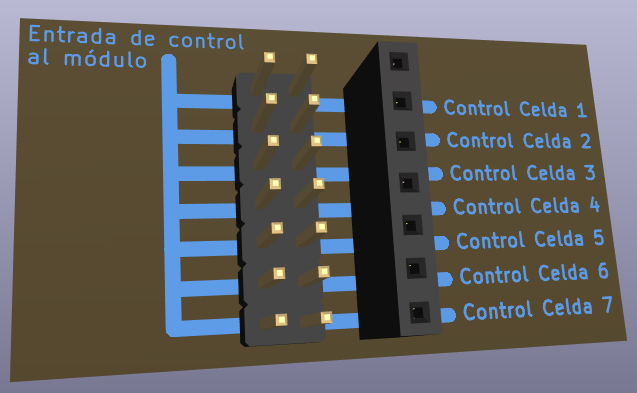
\includegraphics[width=0.75\linewidth]{Imágenes/Diseño final/Celda/Boceto pines de control celdas.png}
    \caption{Configuración realizada para la entrada de las señales de control en cada módulo de celda.}
    \label{fig:pines_control_celda}
\end{figure}

En celeste está diagramado el conexionado entre las dos tiras de pines. Importante destacar que el lado izquierdo de la tira de pines macho doble no está conectado con el lado derecho. Pero los pines del lado izquierdo sí están conectados todos entre sí, los cuales son la señal de entrada al módulo en cuestión. De esta forma, mediante un \textit{jumper} puede seleccionarse cuál de las siete entradas termina siendo la que realmente controla la celda.

Por otro lado, también se tienen las salidas de censado. Se decidió tomar el valor de tensión de cada módulo de celda el valor de $cell\_neg$, es decir, el nodo entre el terminal negativo del portapilas y el \textit{drain} del N-MOSFET. Se utilizó un sistema igual que para las entradas de control: cada módulo tiene las tensiones de todos los módulos del banco. Mediante un \textit{jumper} es que se le asigna a cada módulo su salida correspondiente de entre los siete posibles. Para colocarlo se usa otra tira de siete pines macho dobles.

Con todo esto ya quedan definidas las entradas y salidas de cada módulo de celda. Se tienen veinte pines dobles hembra-macho de entrada/salida:
\begin{itemize}
    \item Pin Vcc.
    \item Dos pines GND. Son dos para facilitar el ruteo (si no habría que usar más vías).
    \item $bus\_pos$.
    \item $bus\_neg$.
    \item Pin de control para todos los módulos del banco $Vcontrol\_global$.
    \item Siete pines de control individual (uno por módulo de celda en el banco).
    \item Siete pines de censado de $cell\_neg$ (uno por módulo).
\end{itemize}

Luego está el tema de la estabilidad mecánica de la torre. Ya se mencionó que el agarre de los pines hembra-macho es fuerte. Sin embargo, para mayor seguridad, se tomaron dos medidas. En un principio, en cada ocasión que se utilizaron dichos pines, se tomaron siempre tiras dobles. De esta forma, la cantidad de pines que se conectan entre un módulo y el siguiente se duplica. El único problema de esto es que no se venden en el país pines hembra-macho dobles, por lo que se utilizaron en cada instancia dos tiras simples (salvo en un caso por temas de espacio en la placa). Por otro lado, la otra medida para hacer más robusta la torre fue colocar los pines en diferentes lados de la placa. Con estas dos medidas, la torre debería mantenerse firme incluso si se conectara la máxima cantidad de celdas posibles por banco.

Existe otro inconveniente del que hasta ahora no se habló: la altura de cada módulo. Para ser más específico, la altura del portapilas. El problema reside en que los pines, a pesar de ser mucho más largos que unos hembra comunes, aún así no son más largos que el alto del portapilas. Esto significaría que una celda no podría conectarse con otra por encima. Para solucionar esto se decidió usar otra iteración de los mismos pines. Es decir, entre módulo y módulo hay otras tiras de pines como se ve en la figura \ref{fig:celda_stackeada}. De esta forma, hay un muy pequeño espacio entre cada módulo, por donde entran sin problema los componentes SMD del circuito.

\begin{figure}[H]
    \centering
    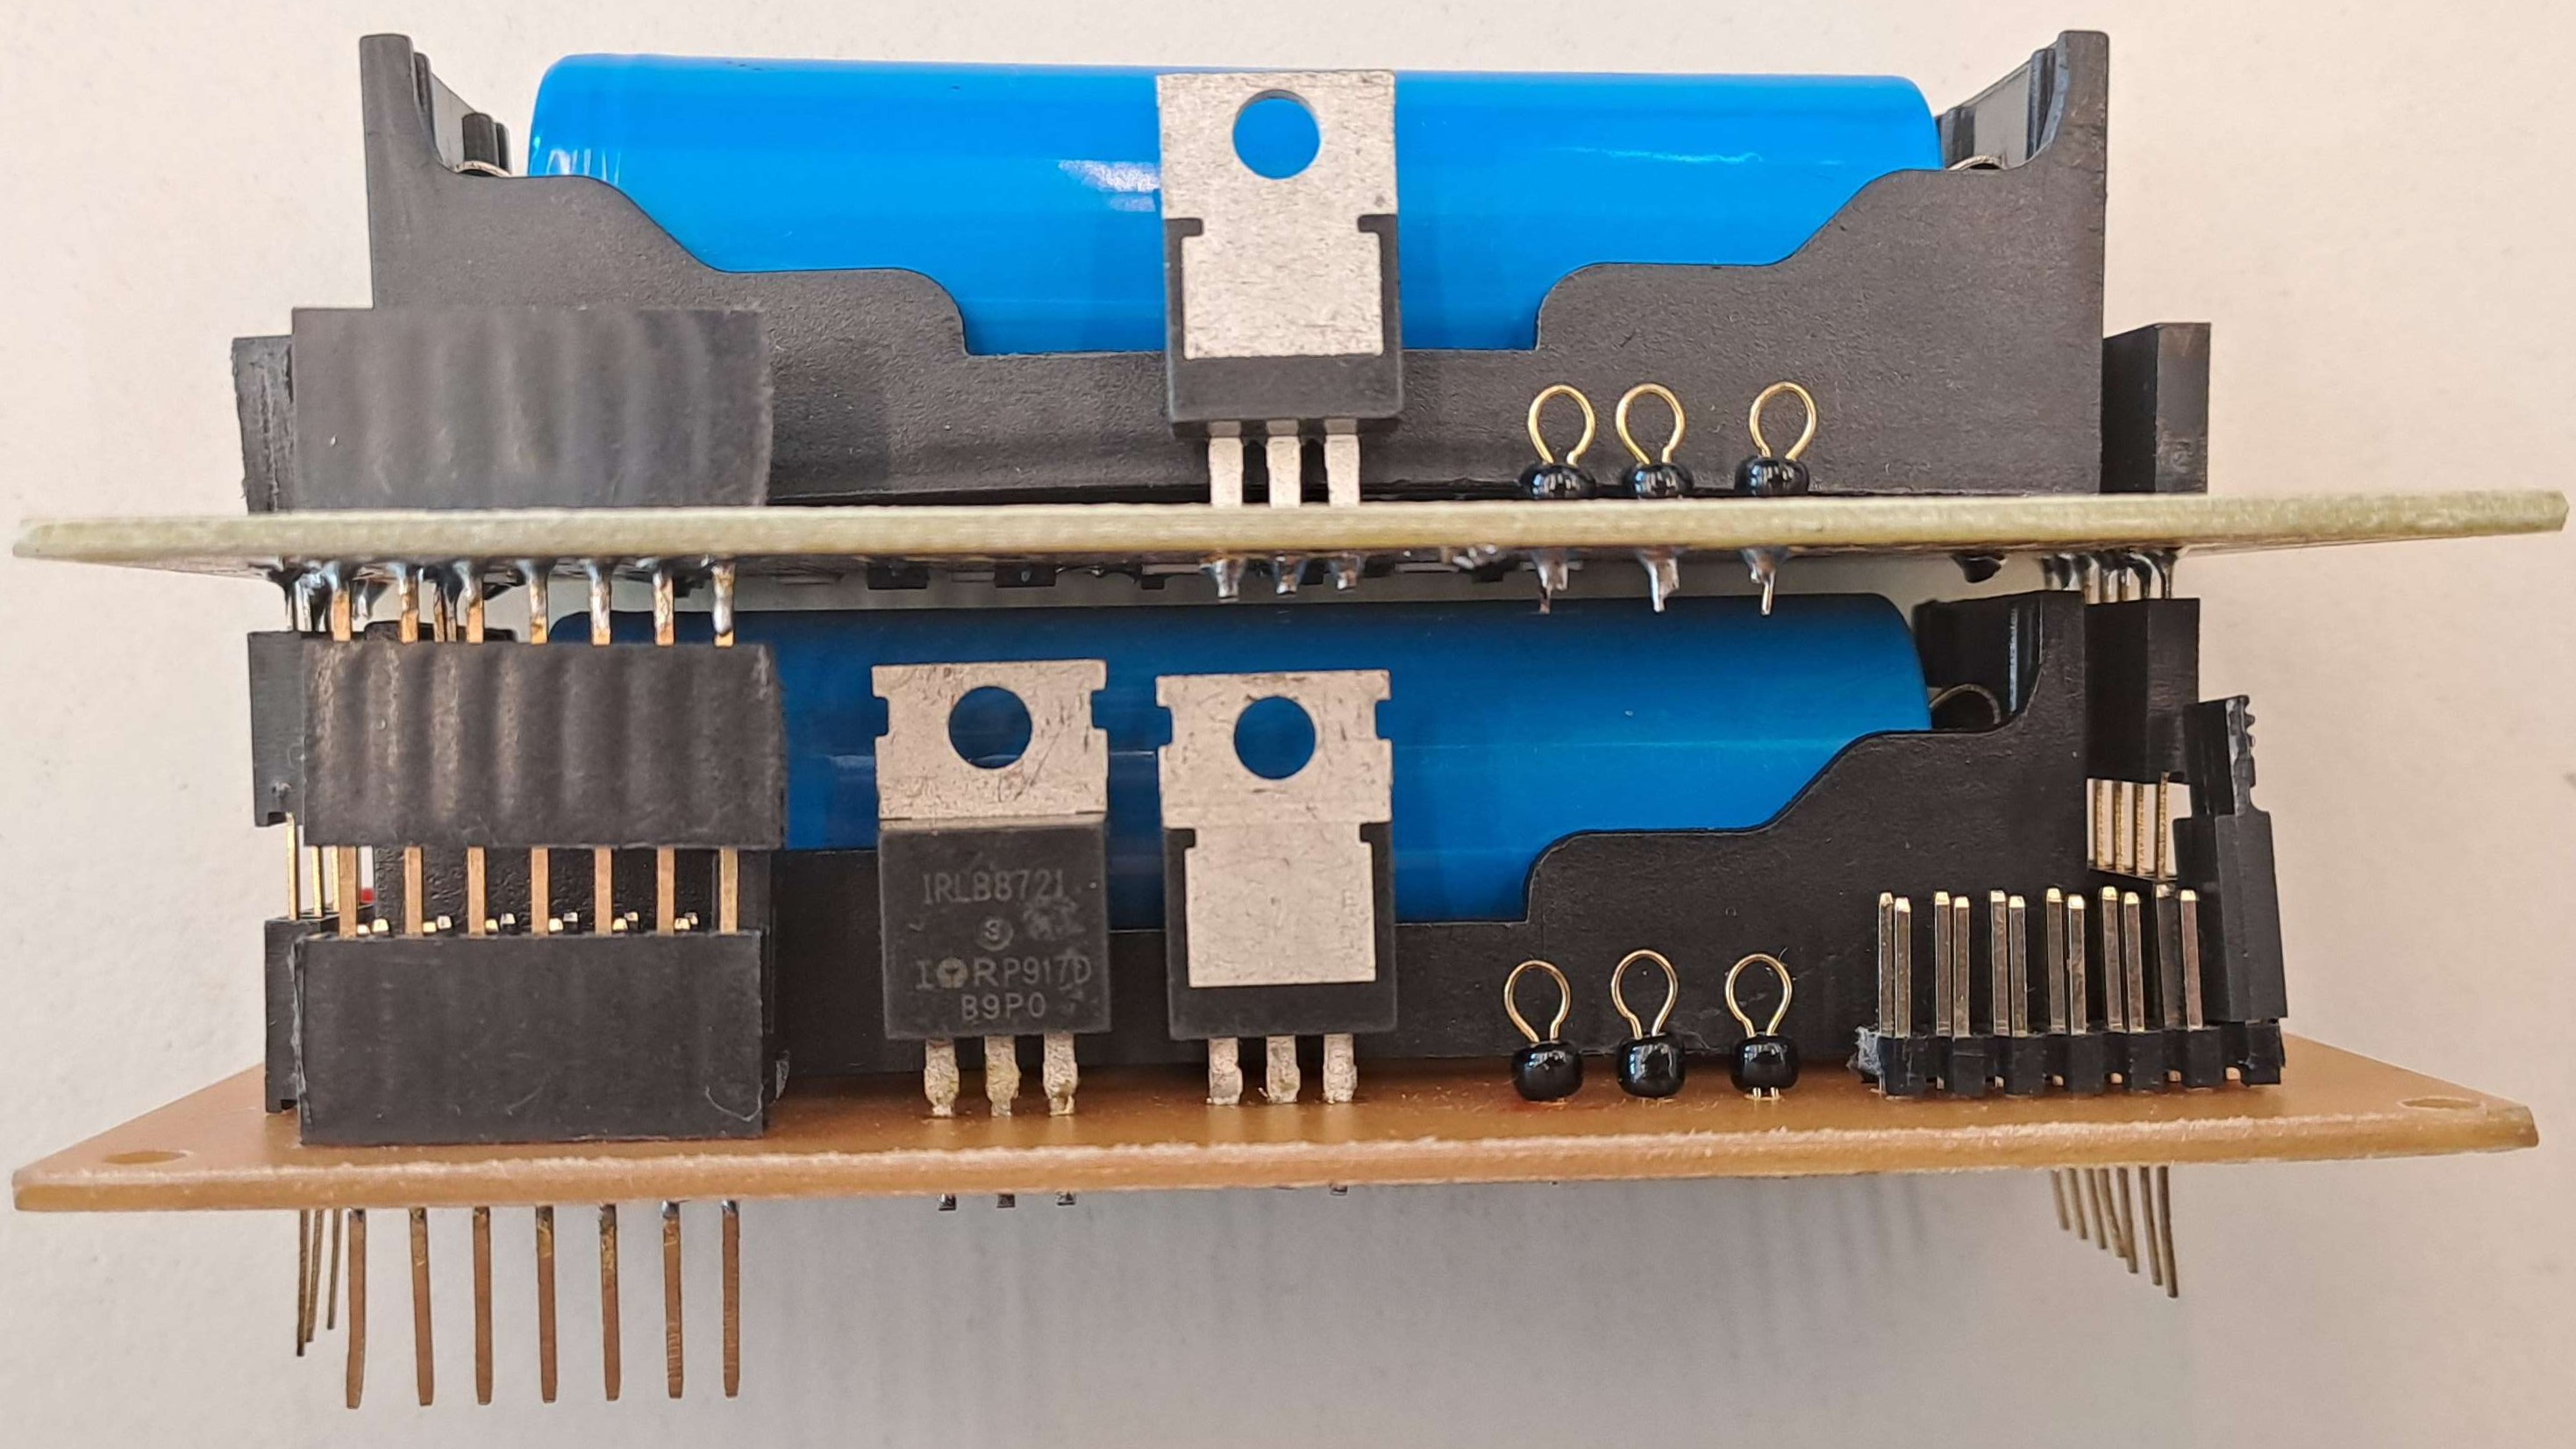
\includegraphics[width=0.75\linewidth]{Imágenes/Diseño final/Celda/Celdas stackeadas.jpg}
    \caption{Dos módulos de celdas (versión 2.1), una por encima de otra, con los pines de conexión.}
    \label{fig:celda_stackeada}
\end{figure}

Como datos de color, se menciona que el MOSFET de canal N que enciende y apaga cada celda se colocó con la cara metálica del encapsulado apuntando hacia afuera de la placa. Esto permite que tenga lugar disponible en caso que se desee incorporar un disipador. No es necesario para esta topología pero, en caso de querer aumentar la corriente a la salida, puede hacer falta. Por otro lado, también se utilizó, como en el prototipo, un fusible de \SI{3}{\ampere} en cada celda en la malla de salida. Además, se creó una pequeña zona libre de cobre en torno a los tornillos sujetadores del portapilas. Esto se hizo para que las tuercas que ajustan no estén en contacto con el plano de tierra del circuito.

En cuanto al ancho de las pistas, se tomó para las pistas de la malla de potencia \SI{1.5}{\milli\meter} y para las pistas de la etapa de control, \SI{0.4}{\milli\meter}. Ambas fueron elegidas de forma tal que puedan sin problemas tolerar la corriente máxima que puede atravesar cada pista. Los valores fueron seleccionados con la tabla dada por Peterson (2025) \cite{peterson2025pcb}.

Finalmente, para facilitar el \textit{debuggeo} se instalaron tres \textit{test-points}: uno en la base del TBJ PNP, otro en el nodo de \textit{gate} del \textit{switch} N-MOSFET y el último a la salida del inversor.

Con todo esto, el circuito resultó como se ve en las figuras \ref{fig:pcb_celda_v20} y \ref{fig:modelo3d_celda_v20}.

\begin{figure}[H]
    \centering
    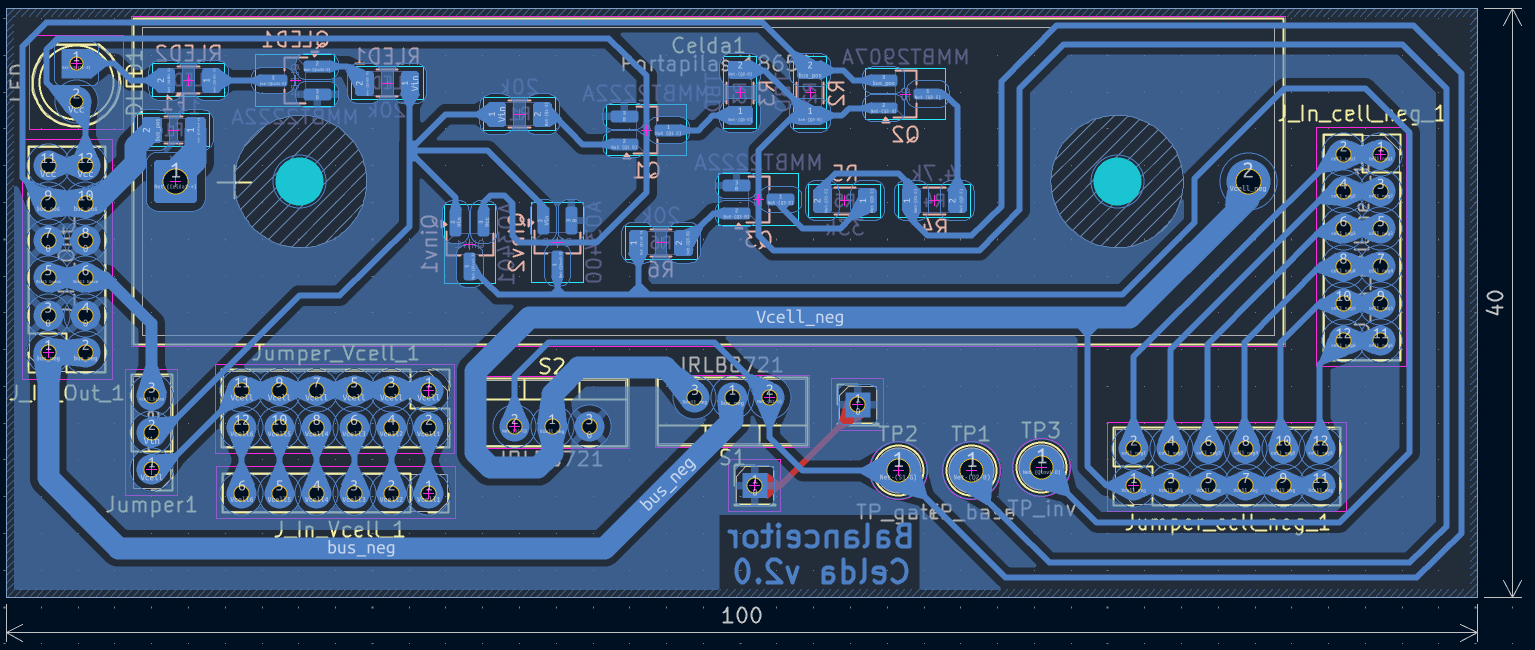
\includegraphics[width=1\linewidth]{Imágenes/Diseño final/Celda/PCB Celda final v20.png}
    \caption{PCB diseñado en \textit{KiCad} del módulo de una celda, versión 2.0.}
    \label{fig:pcb_celda_v20}
\end{figure}

\begin{figure}[H]
    \centering

    \begin{subfigure}{\linewidth}
        \centering
        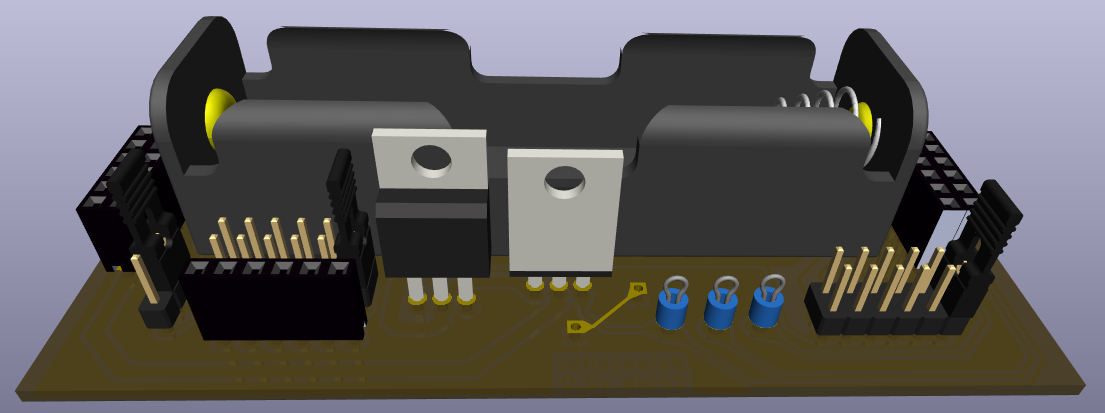
\includegraphics[width=\linewidth]{Imágenes/Diseño final/Celda/Modelo 3D - Celda 2.0 - Front.png}
        \caption{Modelo 3D del frente.}
        \label{fig:modelo3d_celda_v20_f}
    \end{subfigure}

    \vspace{0.5cm}

    \begin{subfigure}{\linewidth}
        \centering
        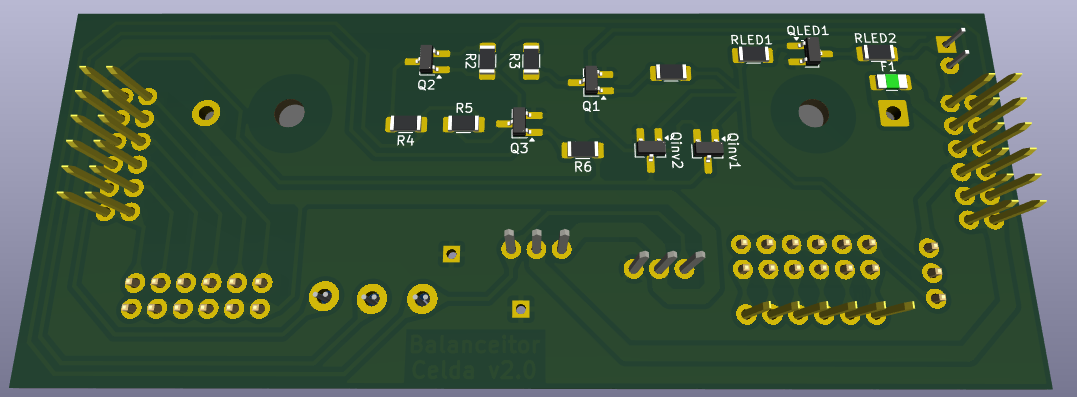
\includegraphics[width=\linewidth]{Imágenes/Diseño final/Celda/Modelo 3D - Celda 2.0 - Back.png}
        \caption{Modelo 3D del reverso.}
        \label{fig:modelo3d_celda_v20_r}
    \end{subfigure}

    \caption{Modelos 3D del módulo de una celda, versión 2.0.}
    \label{fig:modelo3d_celda_v20}
\end{figure}



\subsubsection{Versión 2.1}

La versión 2.0 del módulo de celdas tuvo una vida muy corta. Por un lado, debido a un error de cálculos, se diseñó el módulo para que sea parte de un banco de hasta seis celdas. Sin embargo, el máximo real de módulos conectados que permite el SR es siete. A su vez, hubo un problema mucho más grave: la celda nunca se apagaba. Incluso cuando su señal de control era de apagado, el PNP se mantenía encendido. Esto provocaba un camino de baja impedancia entre el bus positivo y la tierra, mediante los transistores $Q_2$ y $Q_3$ de la figura \ref{fig:circuito_original}. Este problema ya había sido detectado en el prototipo pero se lo había descartado como una falla en la impresión de la placa. Finalmente se encontró la verdadera respuesta, y era efectivamente un problema de diseño. Los resistores $R_2$ y $R_3$, al ser tan grandes ($\SI{10}{\mega\ohm}$ y $\SI{1}{\mega\ohm}$ respectivamente), provocaban una significativa caída de tensión ante cualquier diminuta corriente parásita o de fuga que los atraviesen. Dicha caída era suficientemente alta como para encender el PNP, por ende, encendiendo el N-MOSFET de \textit{switcheo}. Reemplazándolos por resistores de $\SI{100}{\kilo\ohm}$ y $\SI{10}{\kilo\ohm}$ se solucionó el problema. Es curioso notar que este efecto no se veía en simulaciones, dado que era causado por corriente parásitas que el motor del \textit{LTspice} no simula.

Dado que el diseño estaba claramente incorrecto, se creó una nueva versión del módulo de celdas, corrigiendo algunos de los errores encontrados y aplicando otras tantas mejoras.

En un principio, se decidió eliminar el control global de todo el banco del diseño. Se lo consideró innecesario y que agregaba pines y \textit{jumpers} excesivos. Ahora, si se desea apagar o prender todas las celdas de un mismo banco, simplemente se le envía a todas señales iguales en lugar de decidir de qué forma tomar la entrada de control. Esto permitió eliminar el pin de $Vcontrol\_global$ y la tira de tres pines macho con el \textit{jumper} de selección de entrada de control. A su vez, al eliminar este pin de las entradas se simplificó el ruteo, lo cual también se eliminó la necesidad de que hayan dos pines de GND separados.

Por otro lado, hubieron mejoras en cuanto a la estabilidad mecánica de cada torre. En lugar de usar tiras de pines hembra-macho dobles, se instalaron orificios para una varilla roscada de \SI{3}{\milli\meter} en cada esquina de la placa. Así se reemplazaron las tiras dobles por simples, ahorrando en tiras de pines a comprar y espacio en la placa. De esta forma, se tiene ahora certeza absoluta de la robustez de la instalación por las varillas.

Por último, en lugar de una vía se utilizó un resistor SMD de \SI{0}{\ohm}. Éste cumple la misma función pero ocupando menos espacio y sin la necesidad de hacer orificios en la placa.

Con todos los cambios mencionados, también se pudo achicar ligeramente el tamaño de cada módulo (unos pocos milímetros por lado). De este modo, el PCB resultó como se muestra en las figuras \ref{fig:pcb_celda_v21} y \ref{fig:modelo3d_celda_v21}.

\begin{figure}[H]
    \centering
    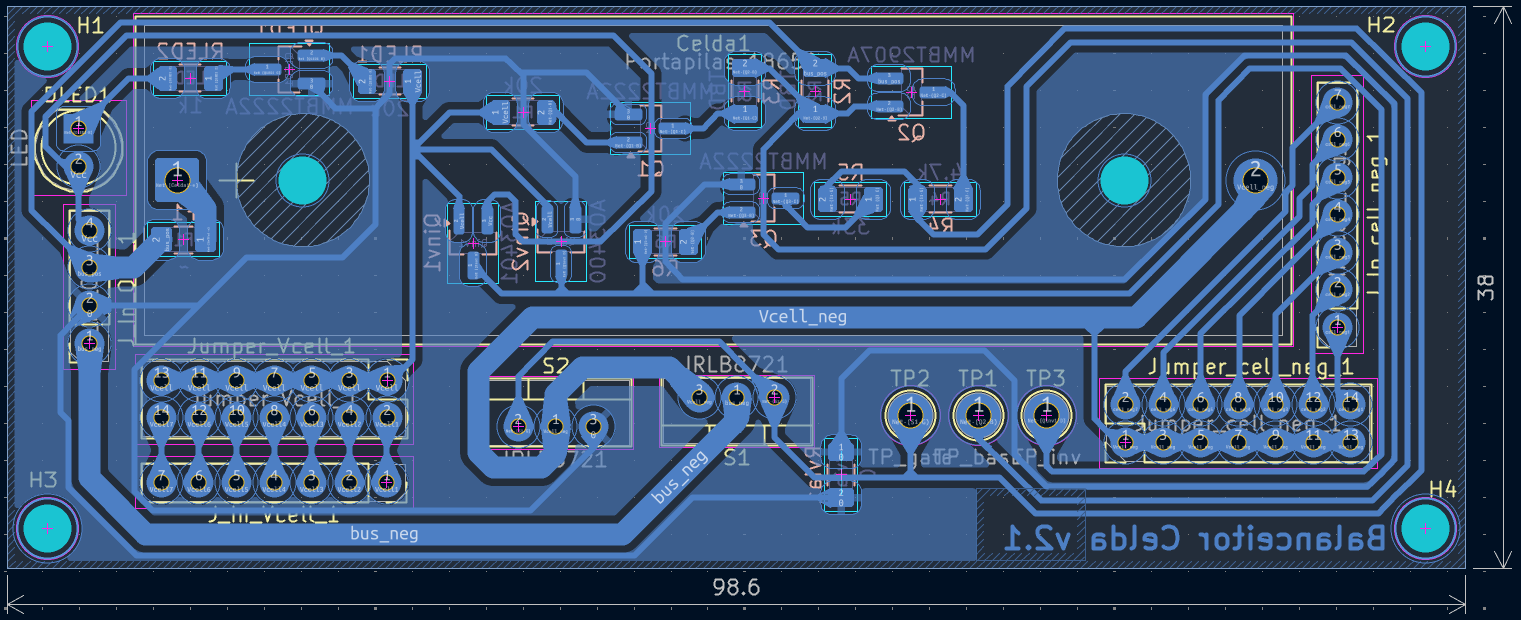
\includegraphics[width=1\linewidth]{Imágenes/Diseño final/Celda/PCB Celda final v2.1.png}
    \caption{PCB diseñado en \textit{KiCad} del módulo de una celda, versión 2.1.}
    \label{fig:pcb_celda_v21}
\end{figure}

\begin{figure}[H]
    \centering

    \begin{subfigure}{\linewidth}
        \centering
        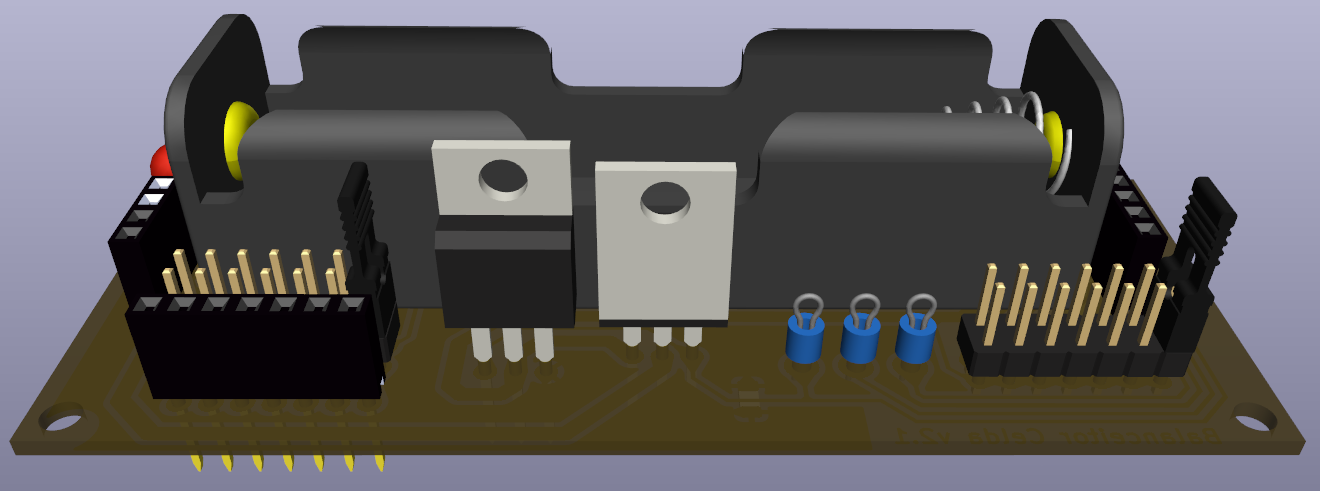
\includegraphics[width=\linewidth]{Imágenes/Diseño final/Celda/Modelo 3D - Celda 2.1 - Front.png}
        \caption{Modelo 3D del frente.}
        \label{fig:modelo3d_celda_v21_f}
    \end{subfigure}

    \vspace{0.5cm}

    \begin{subfigure}{\linewidth}
        \centering
        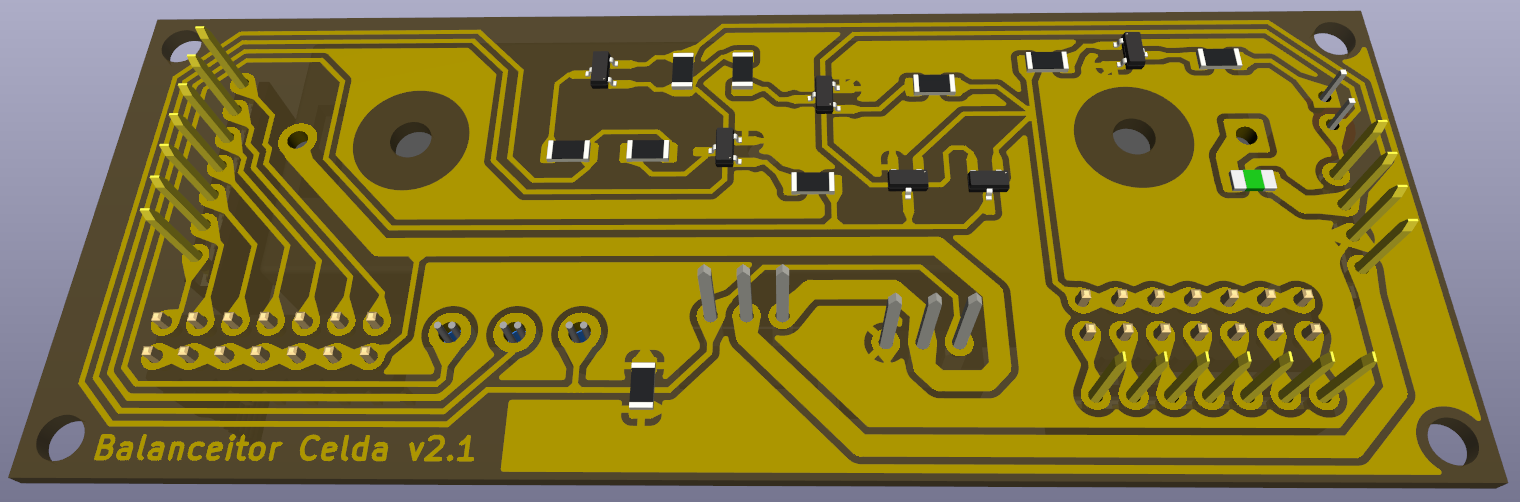
\includegraphics[width=\linewidth]{Imágenes/Diseño final/Celda/Modelo 3D - Celda 2.1 - Back.png}
        \caption{Modelo 3D del reverso.}
        \label{fig:modelo3d_celda_v21_r}
    \end{subfigure}

    \caption{Modelos 3D del módulo de una celda, versión 2.1.}
    \label{fig:modelo3d_celda_v21}
\end{figure}

A diferencia de la versión anterior, esta sí funcionó como era esperado y se cumplieron exitosamente las pruebas básicas de funcionamiento del módulo. Sin embargo, unos resultados fueron algo alarmantes.

\subsubsection{Versión 2.2}

Mientras se realizaban las pruebas de funcionamiento en los módulos de celda v2.1, se descubrió que el valor de tensión de $cell\_neg_1$, el nodo del terminal negativo de las celdas del banco 1, era negativo. Este valor se volvía más negativo a medida que se agregaban más bancos en serie, llegando a unos \SI{-500}{\milli\volt} cuando se tenían cuatro bancos instalados. Esto es alarmante porque ese mismo nodo es el que se censa mediante del multiplexor analógico, el cual, para no dañarse, puede recibir tensiones menores a medio volt negativo. Dado que se está alcanzando dicho umbral, era necesario reducir (en módulo) dicha tensión. Cabe destacar que este fenómeno se da solamente en los nodos $cell\_neg$ de las celdas del banco 1.

\begin{wrapfigure}{l}{0.55\textwidth}
    \centering
    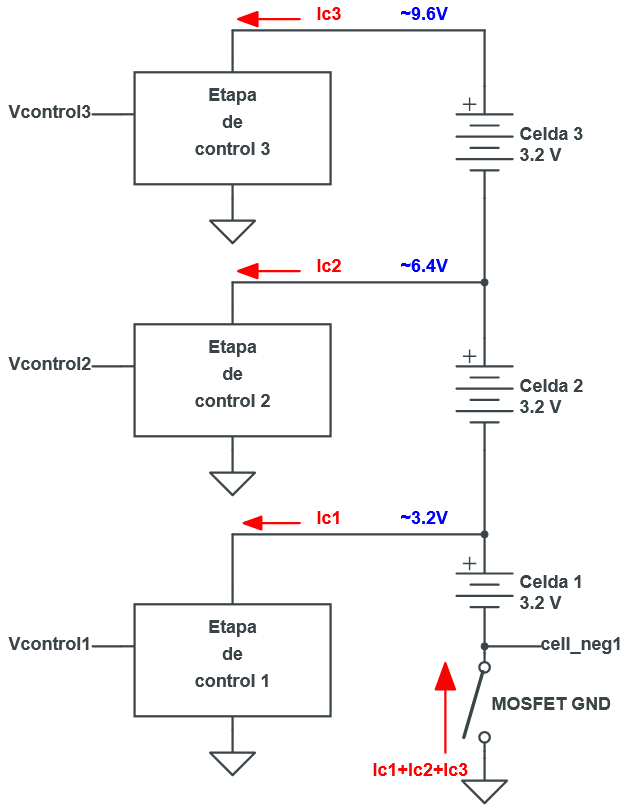
\includegraphics[width=\linewidth]{Imágenes/Diseño final/Celda/Esquema explicación cell_neg negativo.png}
    \caption{Esquema simplificado de un sistema de tres bancos de una celda cada uno.}
    \label{fig:cell_neg_negativo}
\end{wrapfigure}

La causa del problema mencionado se puede analizar de forma más visual mediante el diagrama de la figura \ref{fig:cell_neg_negativo}. El inconveniente radica en que las mallas de control de cada módulo reciben corriente de la misma celda a la que están conectadas y cierran por tierra. 

Esto quiere decir que la única forma en la que la malla se cierra y la corriente regresa a las celdas es mediante la tierra. Cuando el N-MOSFET de GND está cerrado, o lo que es equivalente, cuando la celda del banco 1 está prendida, la corriente retorna sin problema alguno. Sin embargo, cuando dicha celda se encuentra apagada, el MOSFET está abierto. Mediante pruebas empíricas se descubrió que la corriente de todas formas circula a través del transistor, pero con un valor de impedancia significativo. Esto implica una caída de tensión, lo que conlleva a que el nodo $cell\_neg_1$ adquiera un valor de tensión negativo.

Otro dato a destacar es que las corrientes mostradas en el diagrama no son iguales. Su magnitud respeta el ordenamiento $Ic_3 > Ic_2 > Ic_1$ debido a que la caída de tensión en cada etapa de control aumenta a medida que aumenta el número de banco.

Este efecto se tornó mucho más notorio al disminuir las resistencias de $R_2$ y $R_3$. Éstas están relacionadas con la corriente consumida en la etapa de control durante el encendido. La solución no era trivial: se podrían aumentar nuevamente dichas impedancias pero eso significaría regresar el problema que tuvo el módulo v2.0, donde era imposible apagar la celda.

Finalmente se descubrió otra alternativa. Mediante la colocación de un tercer resistor entre $R_2$, $R_3$ y la base del PNP como se muestra en la figura [FIGURA].

% Ton PNP sin Rbase: 210us - Ton PNP con Rbase=100k: 240us

\begin{table}[H]
\centering
\begin{tabular}{@{}cccc@{}}
\toprule
$R_2\ [\Omega]$ & $R_3\ [\Omega]$ & $R_{\text{base}}\ [\Omega]$ & $cell\_neg_1\ [\text{V}]$ \\ \midrule
\SI{100}{k}     & \SI{10}{k}      & 0                           & \SI{-0.510}{} \\
\SI{560}{k}     & \SI{56}{k}      & \SI{100}{k}                 & \SI{-0.428}{} \\
\SI{560}{k}     & \SI{56}{k}      & \SI{560}{k}                 & \SI{-0.280}{} \\ \bottomrule
\end{tabular}
\caption{Comparación de valores de resistencias con su respectivo valor de tensión del nodo $cell\_neg_1$.}
\label{tab:cell_neg}
\end{table}

[SEGUIR]

De esta forma, se diseñó la tercera y última variante del módulo de celda, la versión 2.2 como se aprecia en las figuras \ref{fig:pcb_celda_v22} y \ref{fig:modelo3d_celda_v22}. Como este efecto ya se descubrió que \textit{LTspice} no lo simula, los valores exactos de los resistores no se encontraron hasta que se implementó físicamente el circuito. A su vez, como una alternativa, se instaló un \textit{jumper} soldado para poder cortocircuitar el nuevo resistor $R_{base}$ en caso que se desee regresar a la topología de los módulos v2.1.

\begin{figure}[H]
    \centering
    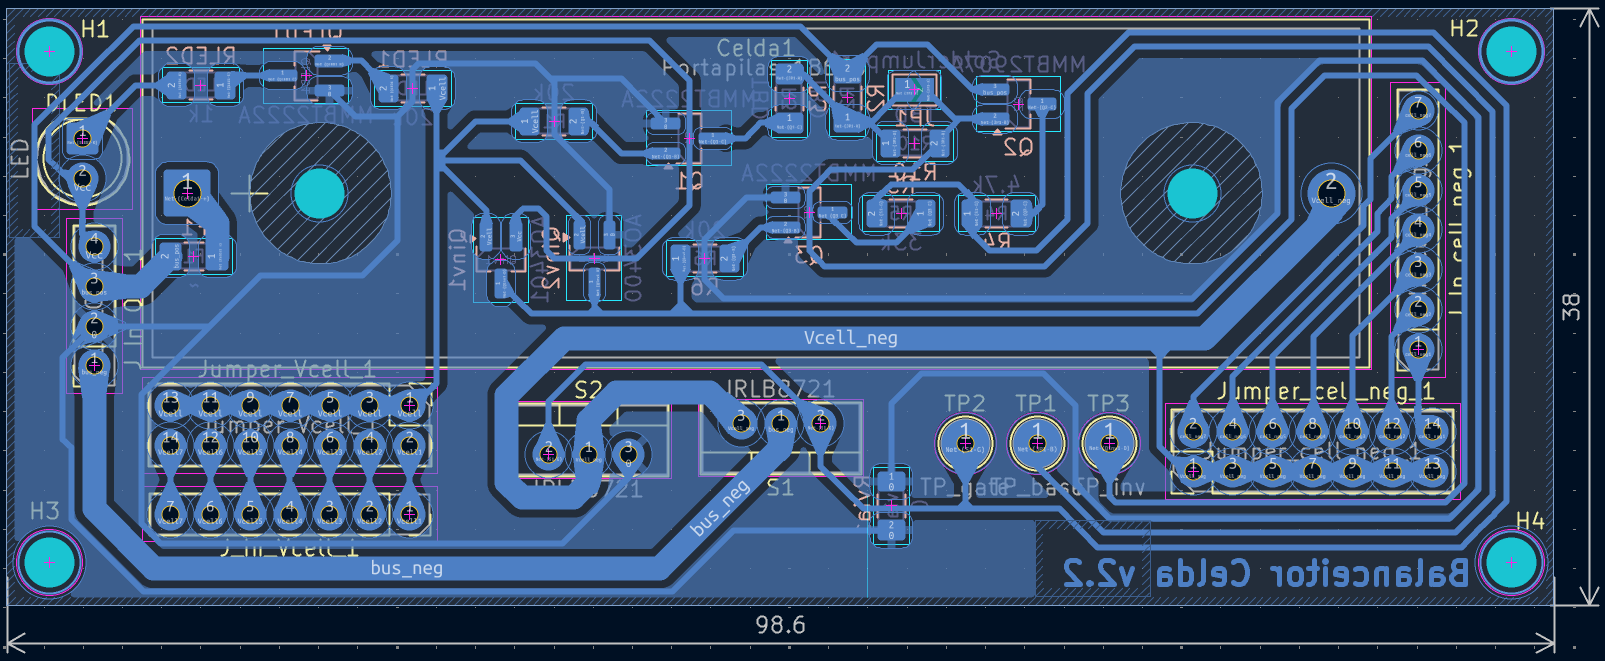
\includegraphics[width=1\linewidth]{Imágenes/Diseño final/Celda/PCB Celda final v22.png}
    \caption{PCB de la versión 2.2 del módulo de celda.}
    \label{fig:pcb_celda_v22}
\end{figure}

\begin{figure}[H]
    \centering

    \begin{subfigure}{\linewidth}
        \centering
        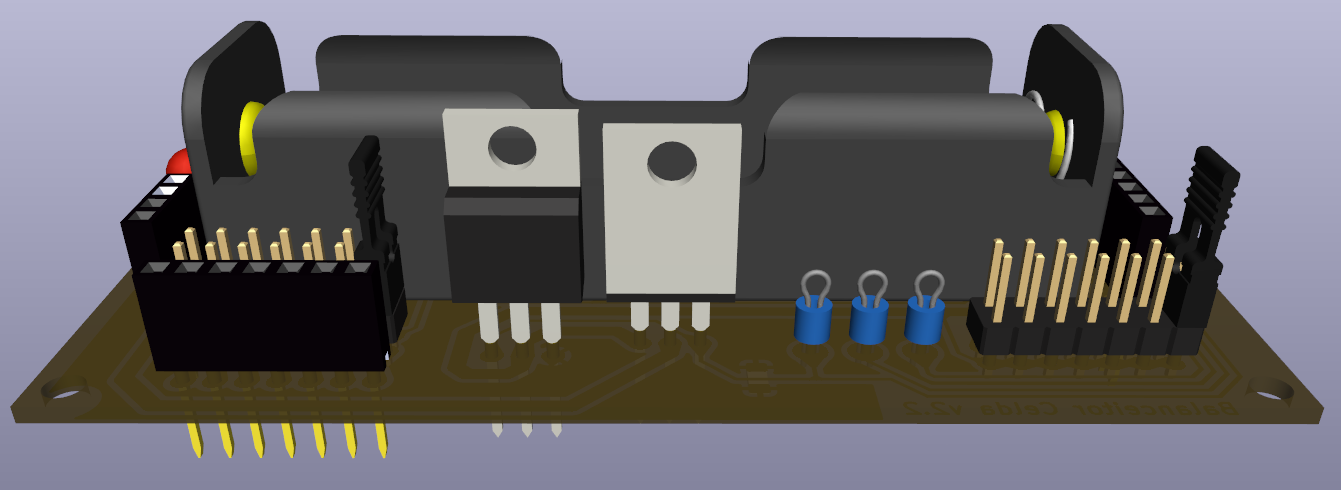
\includegraphics[width=\linewidth]{Imágenes/Diseño final/Celda/Modelo 3D - Celda 2.2 - Front.png}
        \caption{Modelo 3D del frente.}
        \label{fig:modelo3d_celda_v22_f}
    \end{subfigure}

    \vspace{0.5cm}

    \begin{subfigure}{\linewidth}
        \centering
        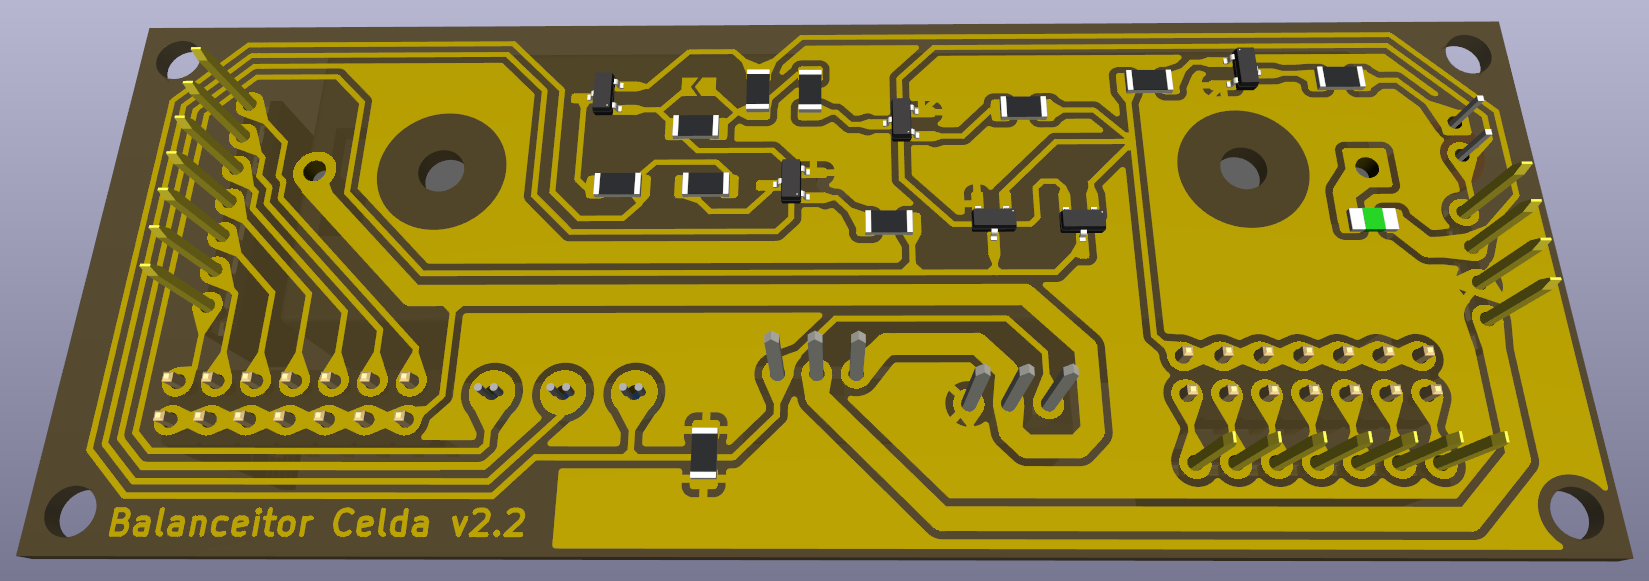
\includegraphics[width=\linewidth]{Imágenes/Diseño final/Celda/Modelo 3D - Celda 2.2 - Back.png}
        \caption{Modelo 3D del reverso.}
        \label{fig:modelo3d_celda_v22_r}
    \end{subfigure}

    \caption{Modelos 3D del módulo de una celda, versión 2.2.}
    \label{fig:modelo3d_celda_v22}
\end{figure}

\subsection{Diseño del circuito de los bancos}

Se comienza con la problemática inicial, el switch de bypass, como se menciona anteriormente el P-MOSFET utilizado en el prototipo, no cumplia con el comportamiento esperado, se vuelve al panorama inicial en la búsqueda de componentes, resultando en dos opciones:

\begin{table}[H]
\centering
\begin{tabular}{@{}cccc@{}}
\toprule
P-MOSFET  & $V_{GS(TH)}\ [\si{\volt}]$ & $R_{DS(on)}\ [\si{\ohm}]$ & $R_{\theta JA}\ [\si{\celsius \per \watt}] $ \\ \midrule
IRLML6402 & -1.2         & 0.065        & 100             \\
AO3401    & -1.3         & 0.085        & 125             \\ \bottomrule
\end{tabular}
\caption{Comparación de criterios para la selección del MOSFET de canal P.}
\label{tab:nuevo_pmos}
\end{table}


 Ambos muy similares pero siendo el \textbf{IRLML6401} con ventaja. Al cambiar a un dispositivo de baja potencia es necesario analizar a la potencia que se verá exigido dicho componente. En este caso se supone una temperatura de funcionamiento  de $\SI{60}{\celsius}$ y del datasheet del componentes se obtiene que $T_{j} = \SI{150}{\celsius}$, se calcula la potencia máxima permitida para el componente con \eqref{eq:potencia_disipada}, obteniendo $P_{permitida} = \SI{900}{\milli \watt}$


\begin{gather}
    P_{permitida} = \frac{T_{jmax} - T_{funcionamiento}}{R_{\theta JA}}
    \label{eq:potencia_disipada}
\end{gather}


A continuación se realiza analiza la potencia en el P-MOSFET del banco 1, aumentando la cantidad de bancos totales, dicho switch siempre encendido y los bancos superiores siempre apagados de forma tal de exponer el switch al caso de mayor exigencia de corriente. Debe destacarse que la carga del sistema se modifica para mantener la corriente constante en la salida en \SI{3}{\ampere} para todas las matrices.



\begin{table}[H]
\centering
\begin{tabular}{@{}ccccc@{}}
\toprule
Cantidad de bancos & $V_{gs} [\si{\volt}]$ & $V_{ds} [\si{\volt}]$ & $I_d  [\si{\ampere}]$ & $Potencia [\si{\milli \watt}[$ \\ \midrule
2                  & -1.86               & -134.6              & -1.5               & 202.8                        \\
3                  & -1.79               & -221.4              & -2.03              & 450.7                        \\
4                  & -1.78               & -250.2              & -2.3               & 577.3                        \\
5                  & -1.767              & -268.0              & -2.47              & 662.47                       \\
6                  & -1.75               & -280.3              & -2.58              & 723.7                        \\ \bottomrule
\end{tabular}
\caption{Potencia en el P-MOSFET en el banco 1 para distinta cantidad de bancos en la matriz.}
\label{tab:potencia}
\end{table}
 



Como se ve en la tabla (\ref{tab:potencia}) este dispositivo disipa energía dentro de los limites establecidos en el datasheet, por lo tanto, para la cantidad de bancos fabricados se cumple con no necesitar disipador. 
De todas formas a modo preventivo en caso de resultar en una potencia mayor en el circuito físico se conecta un segundo P-MOSFET quedando ambos en paralelo. Esto logra dividir la corriente entre ambos MOSFETS, disminuyendo la potencia que disipa cada uno significativamente, en este caso no es de interés que sea una división simétrica de corriente, el único objetivo es no trabajar cerca de la potencia limite. Cabe aclarar que se analiza el caso del bypass del banco 1 ya que es que disipa la mayor cantidad de potencia, en los bancos superiores, la potencia disipada en los bancos superiores resulta menor a los \SI{300}{\milli \watt}.



Ya que el $V_{GS}$ logrado se encuentra cerca del umbral de encendido, el MOSFET opera en una región para la cual el fabricante no especifica el valor de $R_{DSon}$ de funcionamiento. A partir de los valores de la tabla \ref{tab:potencia}, se puede estimar que $R_{DS} = \frac{V_{DS}}{I_D} \simeq \SI{100}{\milli \ohm}$. Por lo tanto al utilizar el esquema de doble P-MOSFET (fig. \ref{fig:doble_pmos}), la resistencia equivalente resulta $R_{DSeq} = \frac{R_{DSon}}{2}$. Por lo tanto no solo  se observa una mejora en cuanto a potencia, al dividirse la corriente en ambos P-MOSFETS, si no que al reducir $R_{DSeq}$, reduce $V_{DS}$ y por consecuencia incrementa ligeramente el $V_{GS}$. Esto significa una menor caida de tensión entre $bus_pos$ y $bus_neg$, resultando en un mejor bypass.  Por otro lado, como buena práctica \cite{ti_mosfet_parallel}, se agrega una pequeña resistencia en el gate de cada MOSFET, asimismo, se busca una conexión simétrica en las pistas que unen a los MOSFETS en el PCB.


\begin{figure}[H]
    \centering
    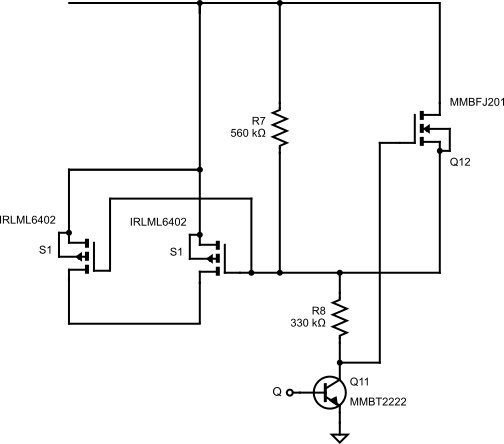
\includegraphics[width=0.75\linewidth]{Imágenes//Diseño final/solo_banco-doble_pmos.png}
    \caption{Conexión del P-MOSFET en paralelo}
    \label{fig:doble_pmos}
\end{figure}



Asimismo se ve en la figura \ref{fig:doble_pmos},  se agrega una resistencia en el gate de cada MOSFET como buena práctica indicada en \cite{ti_mosfet_parallel} y luego en el diseño de PCB se busca asegurar una conexión simetrica en las pistas que unen a los MOSFETS.

Para este modulo, se evalúa la necesidad de utilizar el jfet, se realizan pruebas con solo los elementos del banco en una placa (fig. \ref{fig:placa_de_prueba_banco}).
El principal motivo para agregarlo es para mejorar el apagado del PMOS, un apagado más veloz ayuda a evitar solapamientos entre el PMOS del módulo banco y el NMOS del módulo celda.

\begin{figure}[H]
    \centering
    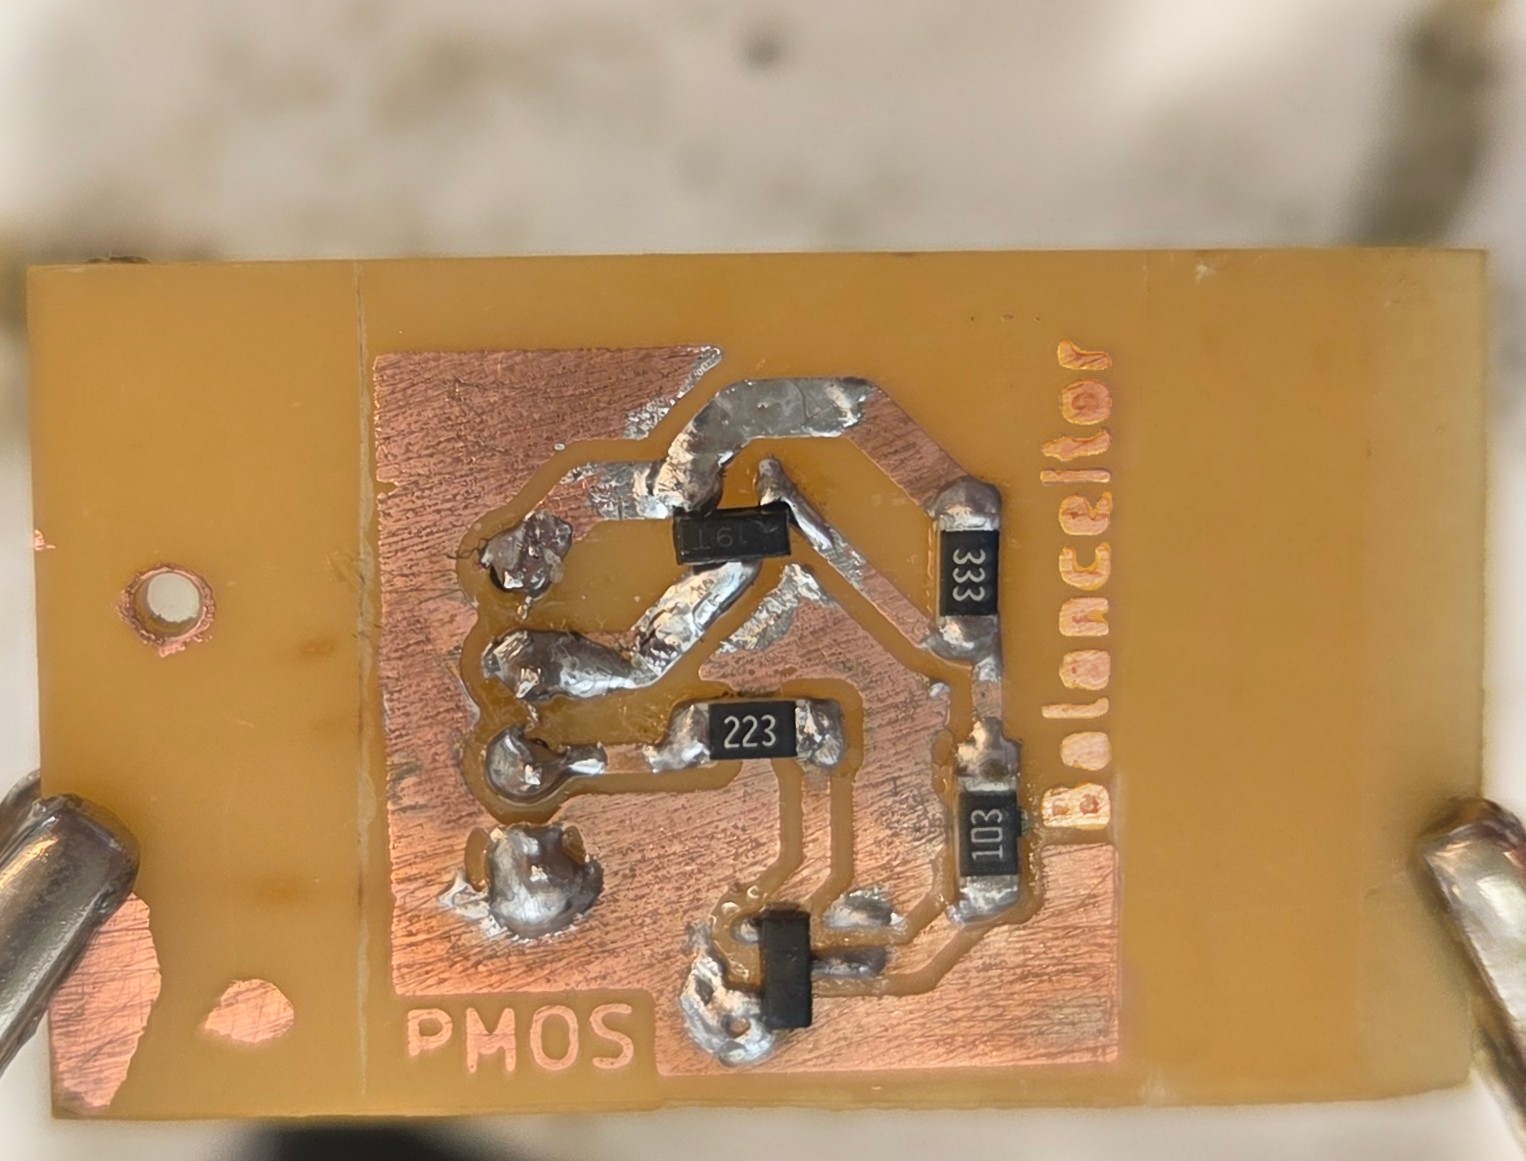
\includegraphics[width=0.5\linewidth]{Imágenes//Diseño final/placa_de_prueba_banco.jpeg}
    \caption{Placa de pruebas de P-MOSFET y JFET.}
    \label{fig:placa_de_prueba_banco}
\end{figure}

Se obtienen as siguientes mediciones:

\begin{figure}[H]
    \centering
    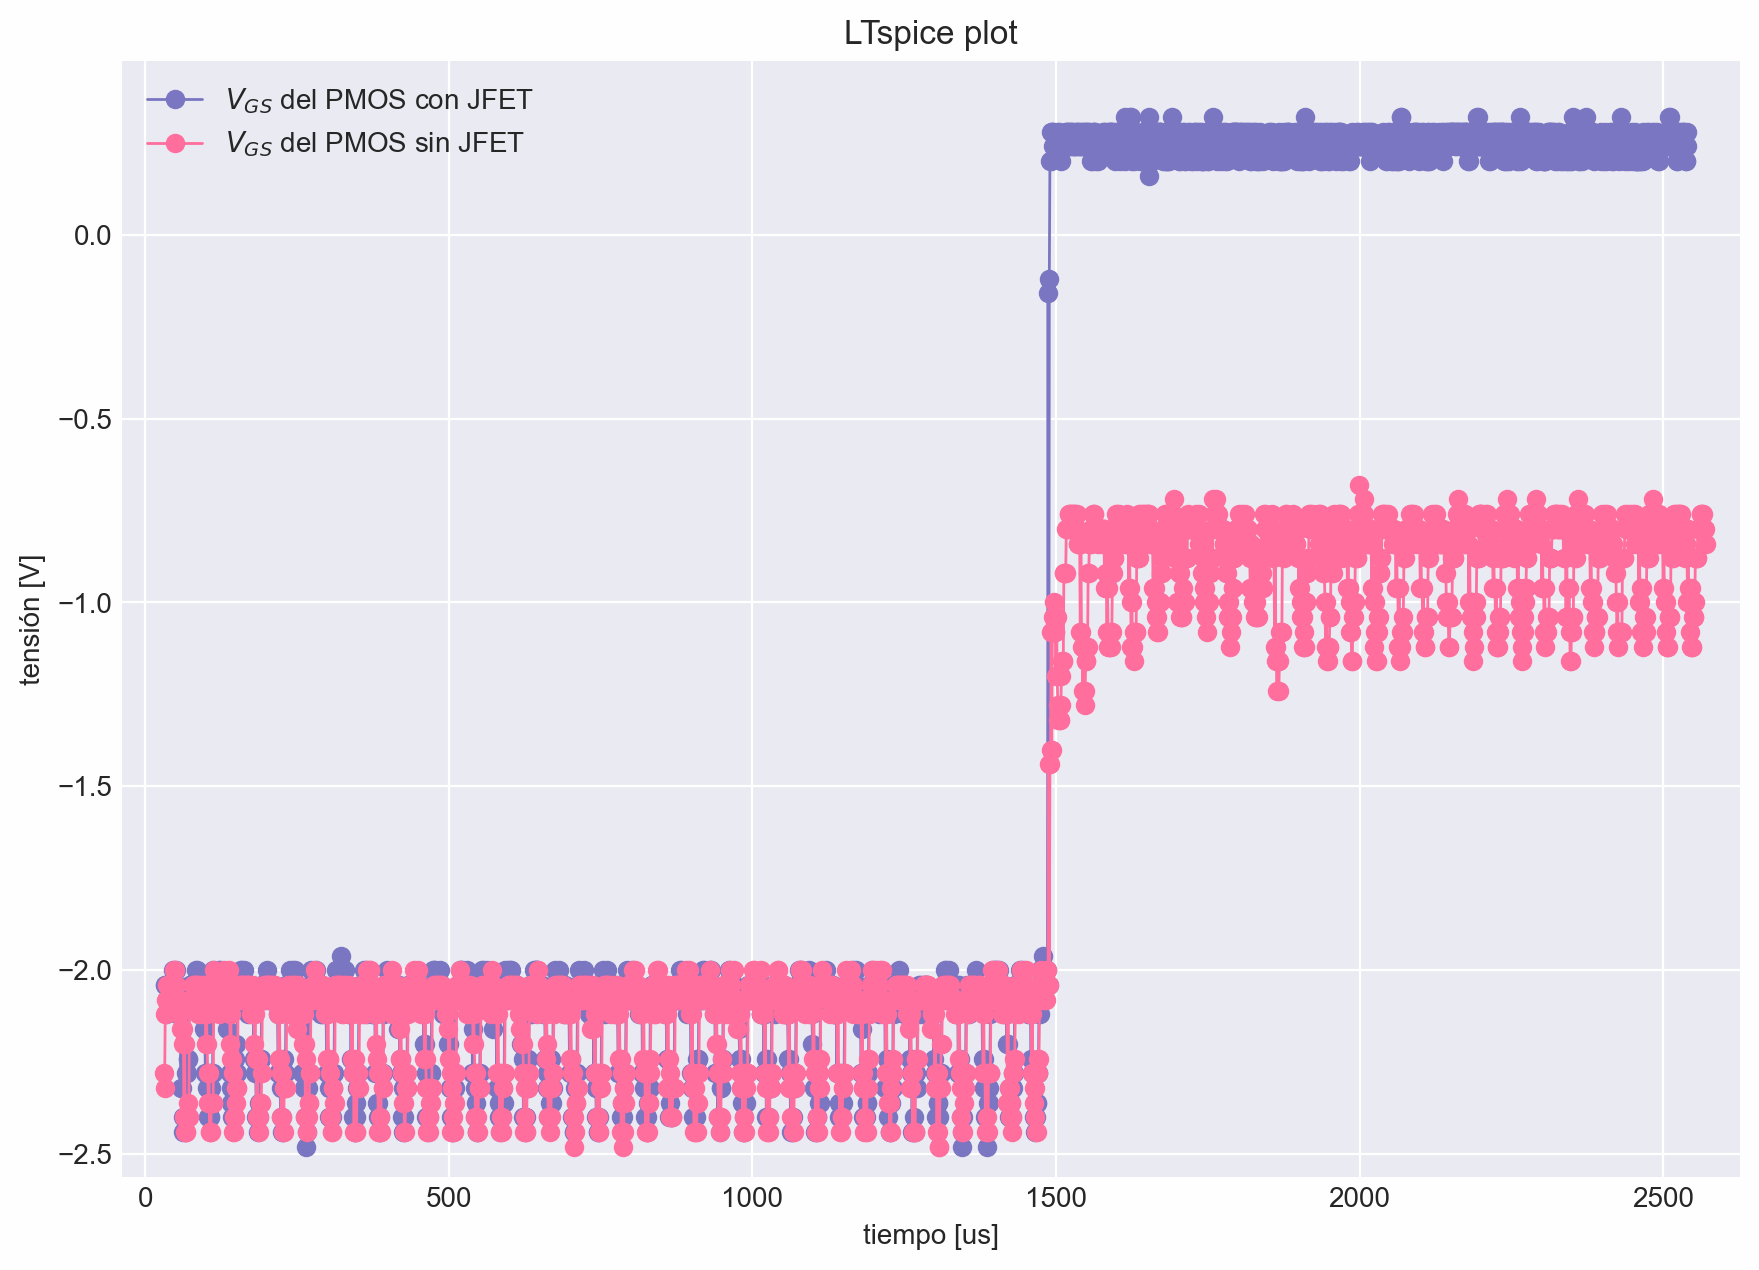
\includegraphics[width=1\linewidth]{Imágenes//Diseño final/vgs comparacion con y sin fet.png}
    \caption{Medición en banco de prueba del $V_{GS}$ del PMOS.}
    \label{fig:vgs comparacion con y sin fet}
\end{figure}


Como se puede observar, es claro el beneficio del JFET. Agregarlo permite que el PMOS pueda efectivamente apagarse, l caso sin JFET se queda en el limite entre el encendido y apagado. En cuanto a la velocidad, son unos pocos \si{\micro \second} de diferencia, pero son los suficientes para provocar un solapamiento con el NMOS del modulo celda. Por lo tanto el módulo banco, continua con JFET.





El modulo banco es el encargado de distribuir las señales de control a las celdas en su dominio. Como se menciona anteriormente, el encargado de realizar esta tarea es el SR, no se exigen criterios exigentes para seleccionar un componente, el componente que más se ajusta al proyecto es el \textbf{74HC595}. Como característica a destacar es que tiene registro de almacenamiento (latch). Este se trata de un componente de 8-bits, el cual permite manejar 8 salidas a partir de 3 señales de entrada. Al enviar la información de las 8 salidas en serie por un solo pin se logra reducir la cantidad de pines de forma significativa. 


Su funcionamiento se basa en dos registros, \textit{registro de desplazamiento}, el cual recibe la información en serie y el registro de almacenamiento, este guarda toda la información y la envía de forma paralela a sus 8 salidas de forma simultanea.
Las señales de control se envían por el pin SERIAL DATA INPUT (DATA), un bit a la vez, de forma simultanea, se  envía un pulso por el pin SHIFT CLOCK. Este último pin al recibir un pulso se encarga de desplazar todos los pines una posición ingresando el bit al registro de desplazamiento. En este estado en las salidas del SR no es posible ver los bits enviados, es necesario enviar un pulso en LATCH CLOCK (LATCH) para enviar todos los bits almacenados.

En cuanto los pines OUTPUT ENABLE (OE) y RESET se conectan directamente a GND y VCC. El primero se encarga de habilitar las salidas en paralelo, esta pin es active-low (entrada negada), por lo tanto se enciende un cero lógico, al colocarlo a GND, las salidas quedan siempre habilitadas. La situación es similar con el pin RESET, es una entrada active-low, por lo tanto un cero lógico resetea el registro de desplazamiento sin modificar las salidas actuales. El pin SERIAL DATA OUTPUT sirve para conectar otros SR en serie, y como las salidas son de alta impedancia, es seguro dejarlo desconectado.





Por lo tanto, para cada banco se necesitan 3 pines para manejar el SR, DATA, CLOCK y LATCH. Para no utilizar pines o señales de control adicionales, se aprovecha  el SR para enviar la señal de control del banco, resultando en 7 salidas paralelas restantes. Este valor es el que se toma como limite de celdas por banco. Como se ve en la figura \ref{fig:sr_conexion}  la primer salida se designa al control del banco y el resto de forma ordenada ascendente a las celdas. A cada salida se le colocan un resistor en serie como protección ante los picos de corriente que se pueden generar debido al inversor en el módulo celda. Para estos resistores se busca que sean valores menores a \SI{500}{\ohm}, su único objetivo es evitar el pico de corriente, no debería haber una gran caída de tensión debido a este.

\begin{figure}[H]
    \centering
    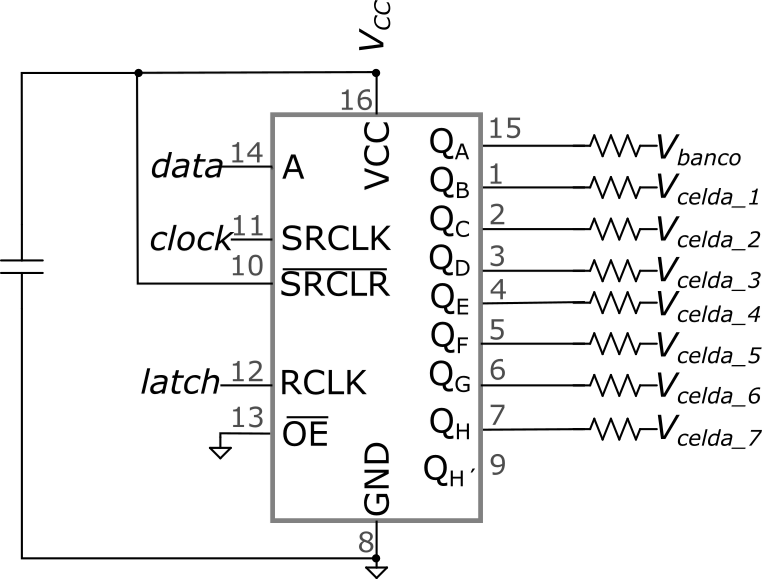
\includegraphics[width=0.75\linewidth]{Imágenes//Diseño final/sr_conexion.png}
    \caption{Diagrama de conexión del SR.}
    \label{fig:sr_conexion}
\end{figure}

En el caso de las mediciones, esta instancia solo se encarga de recolectar las mediciones del terminal negativo de la celda. Este valor no será utilizado en el controlador, pero si debe estar para cumplir con las funcionalidades de la plataforma experimental. Para el presente informe esta medición se encuentra solo como una posibilidad más de medición. Como instrumento de medición se utiliza el \textit{Multiplexor analógico}, \textbf{74HC4051} (MUX). Este componente permite conectar una salida común a uno de los 8 canales analógicos a partir de tres entradas selectoras (S0, S1 y S2). Para este caso, se utiliza como multiplexor, por lo tanto los 8 canales actuan como entradas, y el pin común como salida. La entrada de tensión negativa y el pin que habilita el dispositivo (active-low), se conectan a tierra, permitiendo un rango de tensión para los canales entre $GND$ y $V_{cc}$,y, como en el caso del SR queda constantemente habilitado. 


La entrada del \textit{gpi}o del controlador admite como máximo \SI{3.3}{\volt}, por lo tanto se aprovecha en esta etapa a colocar un divisor resistivo en las canales del MUX. La tensión máxima permitida por el dispositivo es $V_{cc}$ por lo tanto es divisor esta para establecer que la tensión máxima sea  \SI{3.3}{\volt} obteniendo así una tensión que también cumpla con el \textit{gpio} del controlador, La conexión de pines se observa en la figura \ref{fig:diagrama_mux}.

\begin{figure}[H]
    \centering
    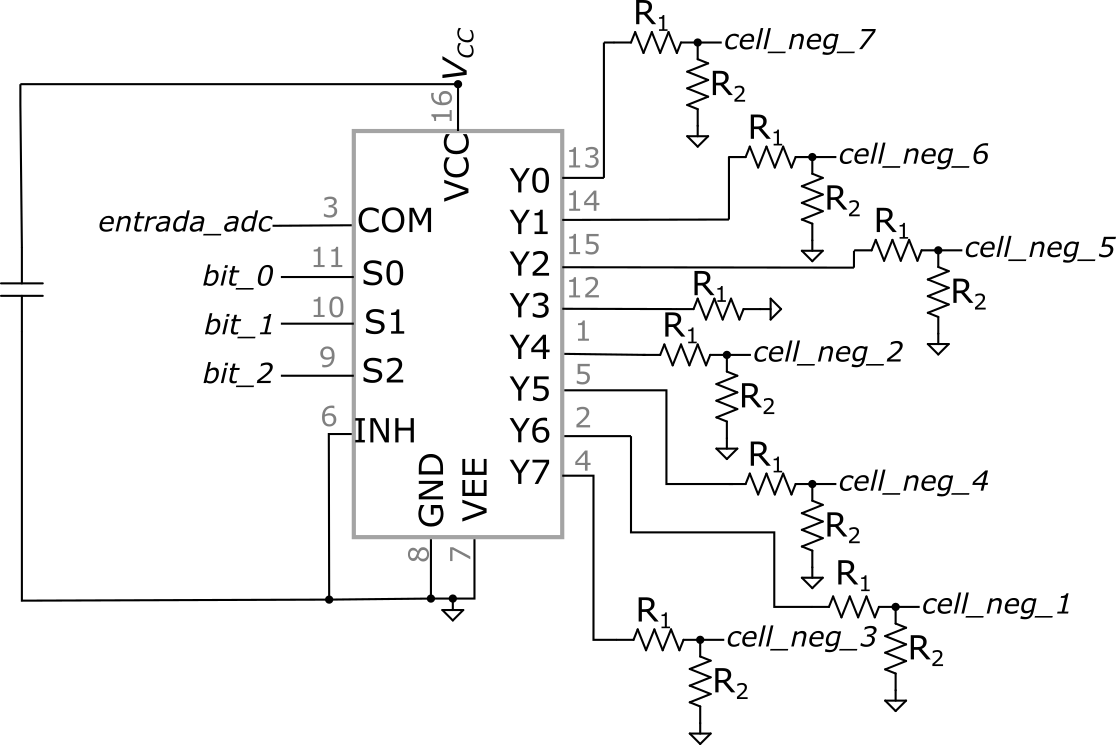
\includegraphics[width=0.75\linewidth]{Imágenes//Diseño final/diagrama_mux.png}
    \caption{Diagrama de conexión del MUX.}
    \label{fig:diagrama_mux}
\end{figure}

Para ambos integrados usados en este módulo se coloca un capacitor de desacople entre $V_{cc}$ y $GND$ para mantener la estabilidad en la alimentación y filtrar ruidos de alta frecuencia. 


Luego para completar el PCB, se coloca el LED correspondiente al banco y los pines  coincidiendo con los pines de la celda. Para la conexión con las celdas se utilizan pines hembra simples. En el caso de las entradas, se busca mejor robustez mecánica por lo tanto se decide utilizar cable plano. Se utilizan pines hembra para cable plano de 14 pines, repitiéndose tan solo $GND$ en dos pines.

El resultado final del PCB se encuentra en la figura\ref{fig:pcb_modulo_banco} El tamaño final resulta por poco un poco más ancho que el modulo celda. Esto incluso resulta favorable para la estructura de torre, ya que proporciona más estabilidad al modulo de celdas cuando la celda ya se encuentra colocada.



\begin{figure}[H]
    \centering
    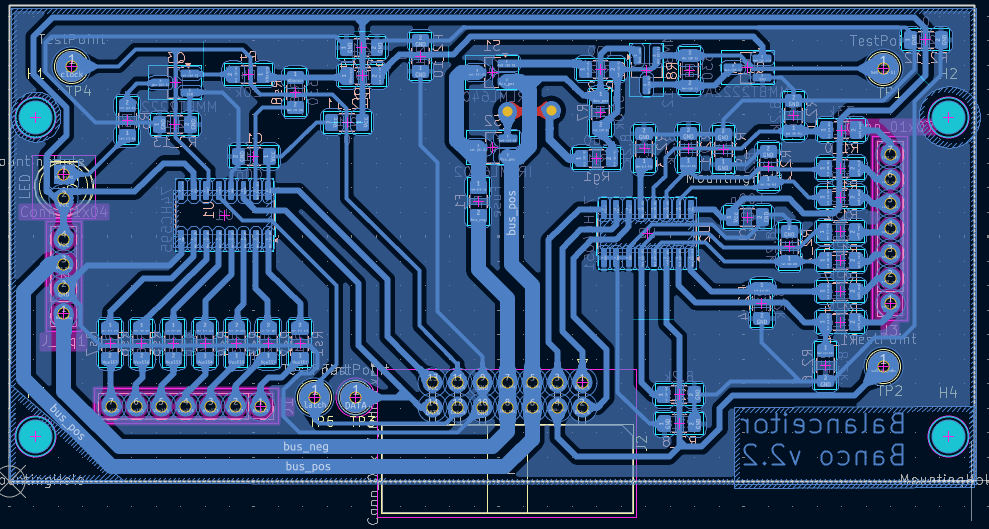
\includegraphics[width=1\linewidth]{Imágenes//Diseño final/pcb_modulo_banco.png}
    \caption{Diseño del PCB del módulo banco,}
    \label{fig:pcb_modulo_banco}
\end{figure}



Para llegar al diseño final del pcb, es decir la \textbf{versión 2.2} (fig. \ref{fig:pcb_modulo_banco}) se realizaron los siguientes cambios:

\begin{enumerate}
    \item Cambio de huellas: El primer error durante la elaboración fue utilizar huellas \textit{DIP-16}, que luego se modificaron por huellas \textit{SOIC-16}. Dando origen a la\textbf{ versión 2.1}. Para esta versión se agregan test points en la salida del mux, y en los pines de control del SR.

    \item El siguiente cambio fue eliminar resistencias de pull down en el shift register, En una versión inicial, se utilizaba el pin $OE$ del SR para la llave maestra por lo cual resultaba necesario que los pines de salida no queden en alta impedancia en caso de deshabilitar las salidas. Dicha idea se decartó y los resistores se eliminaron para una mejor eficiencia del SR en la \textbf{versión 2.2}.
\end{enumerate}


\begin{comment}
    poner imagen del resultado final del banco
\end{comment}


\subsection{Diseño del circuito central}

Como se mencionó previamente, como placa controladora se utilizó una \textbf{STM32 NUCLEO-F103RB}. Haciendo mediciones de testeo, rápidamente se hizo notoria la necesidad de simplificar el conexionado entre controlador y módulos de banco al igual que entre los mismos bancos entre sí. Al haber tantas señales que debían enviarse, muchas digitales y otras analógicas que debían conectarse en pines específicos, se tornaba una tarea muy tediosa cada vez se armaba y desarmaba el sistema. Para esto es que se diseñó el llamado \enquote*{circuito central}. Su tarea era ser simplemente una placa con pines hembra donde se montara la STM32, y tenga salidas mediante conectores de cable plano para enviar a cada módulo de banco. De esta forma, se reemplazaría todo el cableado por ruteo de la placa y las conexiones serían mediante tiras de catorce cables planos.

Originalmente se decidió que la placa no tenga ningún tipo de lógica circuital. Es decir, su rol es únicamente de soporte mecánico y de envío de información mediante buses.

Sin embargo, a medida que se hacían mediciones de pruebas sobre las demás placas, fueron surgiendo la necesidad (e ideas nuevas) con funciones para implementar. Para cuando se diseñó efectivamente la placa, lejos estaba de esa propuesta original muy simple de ser únicamente para simplificar el conexionado. Estas nuevas funciones agregadas fueron:
\begin{enumerate}
    \item Una llave de apagado manual y otra automática.
    \item \textit{Switches} entre cada banco y la salida, y entre bancos.
    \item Un medidor de corriente a la salida.
    \item La creación de una tensión $-Vcc$ de \SI{-5}{\volt}.
    \item Amplificadores operacionales para proteger los pines del controlador que censan tensión.
\end{enumerate}

Con respecto a los \textit{switches}, como se mencionó, hubieron uno manual y otro controlado. Ambos funcionan cortando la llegada de $Vcc$ a los módulos, y de esta forma, evitando cualquier tipo de control sobre las celdas. El manual se implementó con un pulsador y funciona simplemente como un botón de prendido y apagado de todo el sistema. A su vez, el automático se implementó, con la topología mostrada en la figura [FIG], con el objetivo de apagar todo el sistema ante la detección de una falla crítica (como puede serlo, un pico demasiado alto de corriente).

[AGREGAR DIAGRAMA DEL SWITCH PMOS]

[COMPLETAR]

\subsection{Problemas de diseño} 

Uno de los principales problemas durante el diseño del circuito inicial fue la tierra, colocando una tierra virtual en el terminal negativo se logra que funcione el sistema, pero se encontraron algunos inconvenientes. Se utiliza como banco de prueba una matriz de $2x1$, dos bancos de una celda y se observaron los siguientes resultados:


\begin{itemize}
    \item Banco 1 OFF, Banco 2 ON,
    \begin{figure}[H]
        \centering
        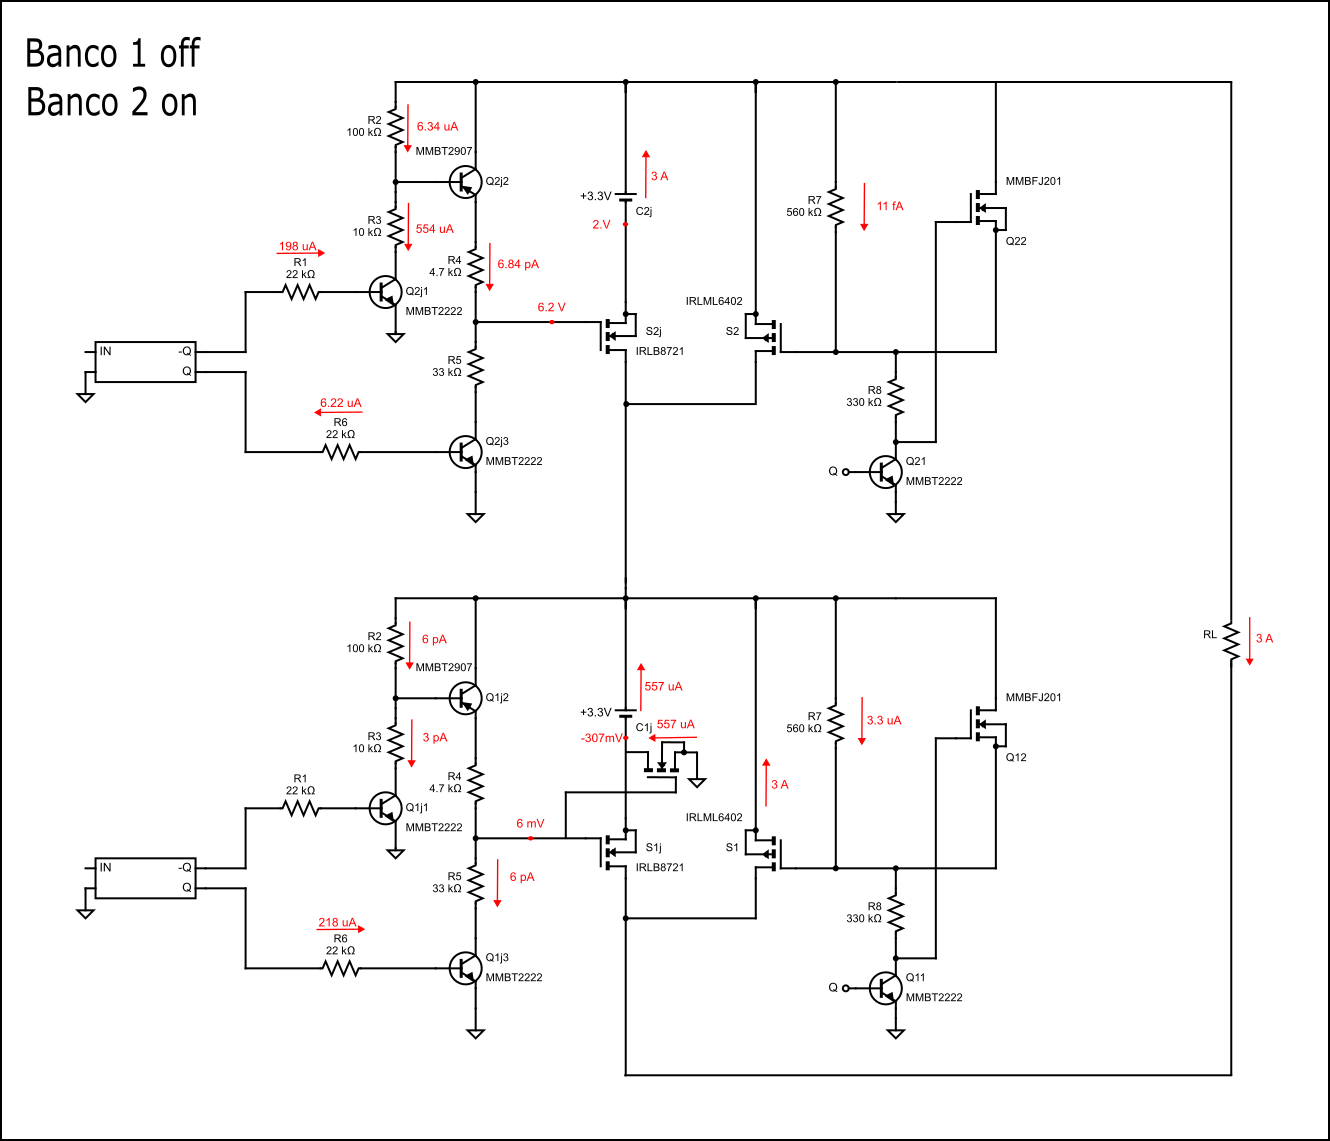
\includegraphics[width=0.75\linewidth]{Imágenes//Diseño final/banco1_off_b2on.png}
        \caption{ Análisis de corriente para la configuración: \textit{Banco 1 OFF, Banco 2 ON}}
        \label{fig:banco1_off_b2on}
    \end{figure}
    

    \item Banco 1 ON, Banco 2 OFF,
    \begin{figure}[H]
        \centering
        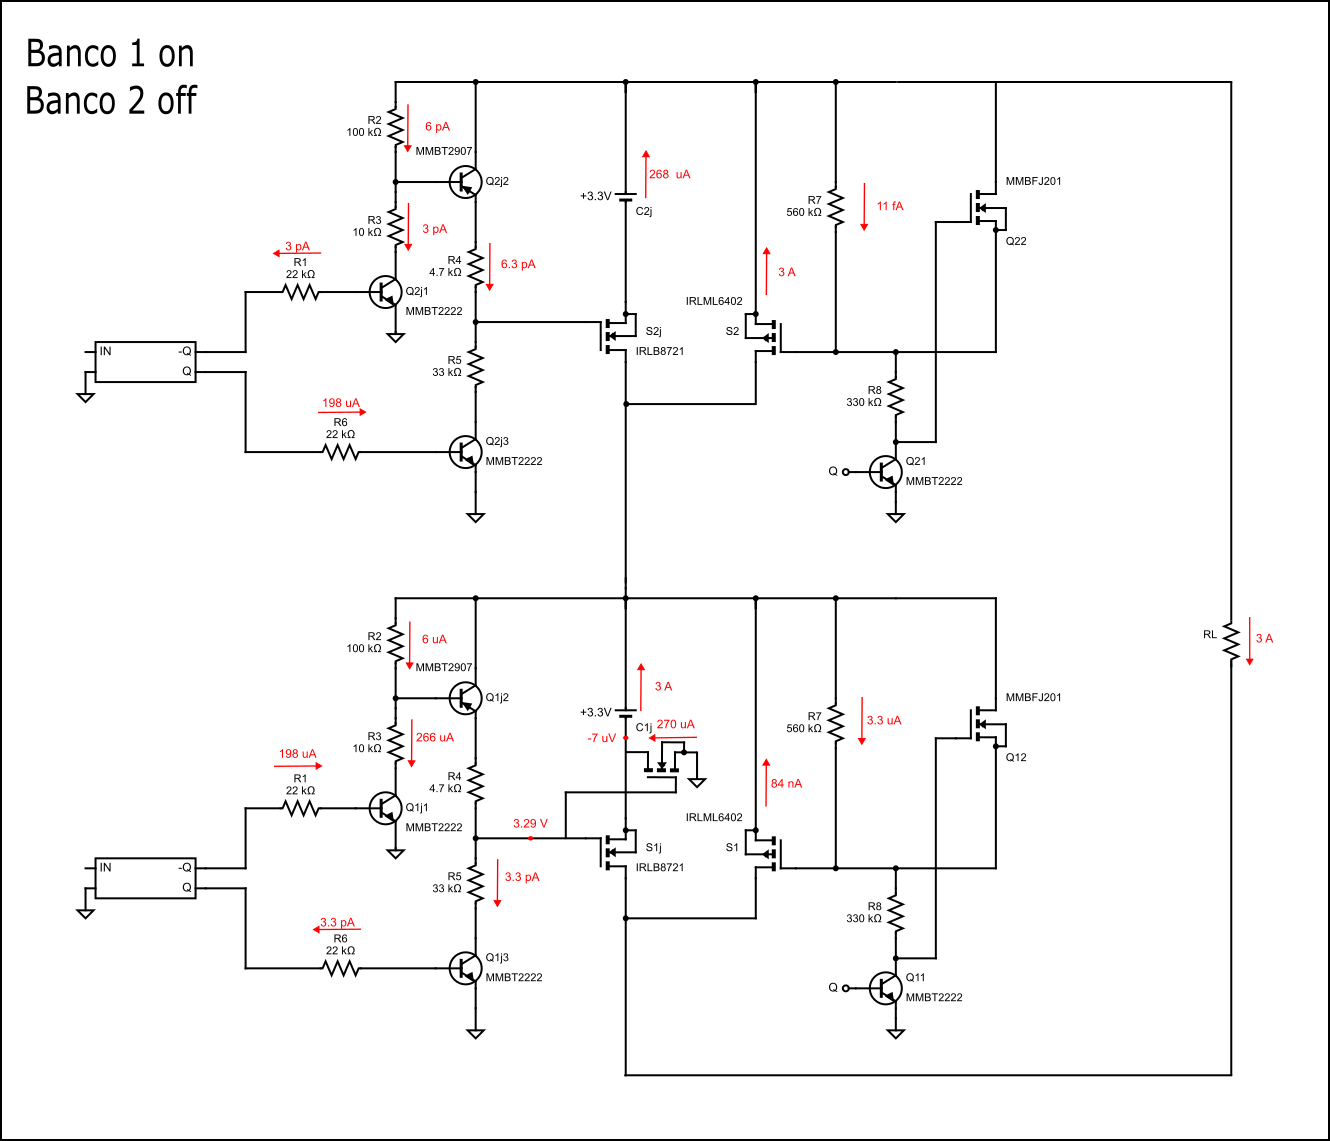
\includegraphics[width=0.75\linewidth]{Imágenes//Diseño final/banco1_on_b2off.png}
        \caption{Análisis de corriente para la configuración: \textit{ Banco 1 ON, Banco 2 OFF}}
        \label{fig:banco1_on_b2off}
    \end{figure}
    \item Banco 1 ON, Banco 2 ON,
    \begin{figure}[H]
        \centering
        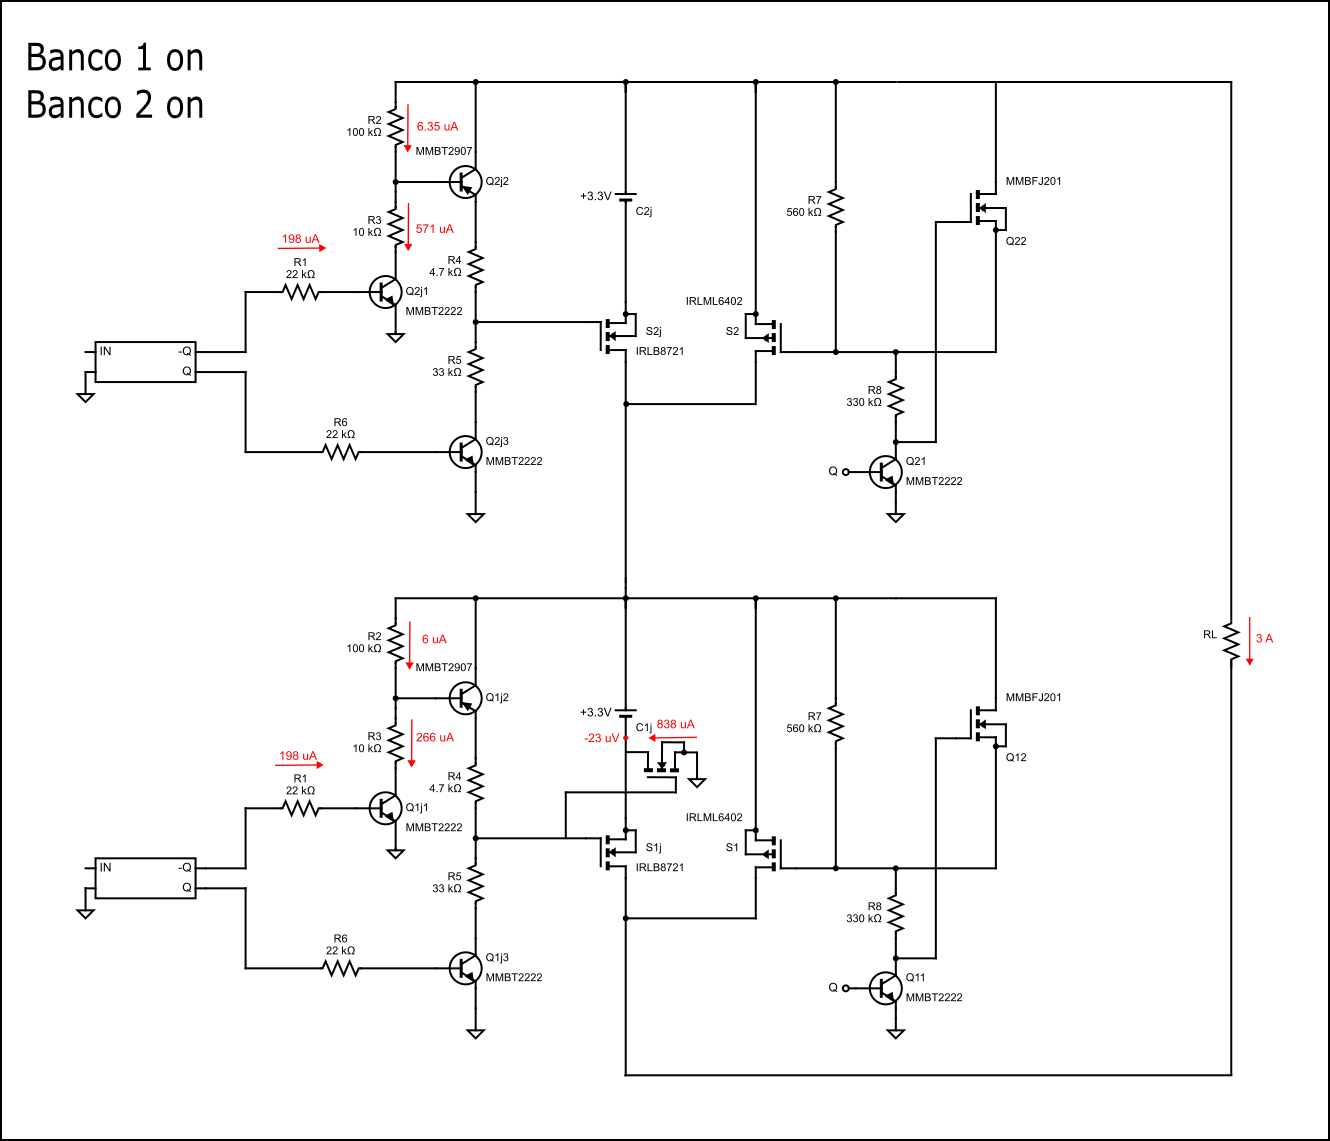
\includegraphics[width=1\linewidth]{Imágenes//Diseño final/banco1_on_b2on.png}
        \caption{Análisis de corriente para la configuración: \textit{Banco 1 ON, Banco 2 ON}}
        \label{fig:banco1_on_b2on}
    \end{figure}
    
\end{itemize}
Lo primero en notar de esta situación (fig. \ref{fig:banco1_off_b2on}) es la corriente en el MOSFET de tierra, esto provoca una tensión negativa en el terminal negativo de la celda. Analizando la corriente en cada componente del circuito de la celda, es posible notar que dicha corriente se genera en el driver del banco 2. Al encender la celda del banco 2, es decir encender el TBJ NPN $Q_{2j2}$, el colector queda a tierra, cerrando la malla atraves de la tierra virtual del MOSFET de tierra. Como no hay una referencia a GND para cada banco, al agregar bancos aumenta la tensión que percibe el driver de dicho banco, resultando en un aumento de corriente en el colector del TBJ de encendido.

Como se ve en (fig. \ref{fig:banco1_on_b2off}), y en (fig. \ref{fig:banco1_on_b2on}), este efecto ocurre incluso en caso de estar el banco 1 encendido. Al estar la celda del banco 1 encendida, se produce el efecto de la tierra virtual obteniendo que la celda tenga su terminal negativo a GND, pero al medir la corriente que circula en el MOSFET de tierra, se sigue viendo lo descripto anteriormente. Esto principalmente ocurre por que hay un único GND global para todo el circuito y la tierra virtual resulta ser el mismo. 





\subsection{Diseño del controlador}

Para el controlador de este diseño modular, no es posible partir del controlador del prototipo, es necesario un nuevo planteo. Los principales cambios son debido al \textit{hardware}, los cuales afectan a la lógica del software. 

Toda la lógica de encendido ahora depende del SR, a diferencia del controlador del prototipo donde cada switch era un pin del \textit{GPIO}. acá solo hay un pin de \textit{Data} y es el SR el que se encarga de seleccionar el switch a accionar. A cada banco le corresponde un switch, y a modo de mantener todo sincronizado y ahorrar pines \textit{GPIO}, se decide que los pines del SR \textit{Latch} y \textit{Clock} serán los mismo para toda la matriz. Esto implica que cada vez se envía un pulso de \textit{clock} el bit actual en data de todos los bancos será desplazado, de igual manera con un pulso de \textit{latch}. Por lo tanto hay que tener precaución  al enviar los pulsos de \textit{latch} y \textit{clock} para evitar enviar información basura a los \textit{switches}.

Por lo tanto, ahora se organiza el controlador por jerarquías. Se siguen mandando las instrucciones por \textit{USART}, y el que las maneja es el \textbf{controlador} el cual tiene un conjunto de bancos, a cada banco le asigna un SR. Desde el banco solo se va a poder enviar un '1' o un '0', pero sin activar el \textit{clock}, es el controlador el que se va a encargar de los mandar pulsos de \textit{clock} y \textit{latch} solo cuando todos los pines de data

\section{Posibles mejoras}

\begin{itemize}
    \item Resistores de la salida del SR en cada celda en lugar del banco.
    \item Resistor chiquito de protección en el inversor de cada celda.
    \item Implementación de micro por celda para poder usar protocolos de comunicación más sofisticados (y eliminar los jumpers).
    \item Implementación de tensión negativa en cada banco (ya sea mediante otra entrada o un ICL) para que el MUX pueda correctamente medir el valor de $cell\_neg$.
    \item Switches entre bancos y dip switches entre bancos y salida automáticos.
    \item Implementación de integrado para censado de corriente bidireccional.
    \item Implementación de $Vcc$ a partir de la batería misma.
\end{itemize}





\newpage
\bibliographystyle{IEEEtran}
\bibliography{biblio}

[AGREGARLE COMO REFERENCIAS LAS HOJAS DE DATOS]

\end{document}